\documentclass[12pt,openany]{mitthesis}
\setcounter{tocdepth}{3}% Include \subsubsection in ToC
\setcounter{secnumdepth}{3}% Number \subsubsection
\usepackage{lgrind}
%% These have been added at the request of the MIT Libraries, because
%% some PDF conversions mess up the ligatures.  -LB, 1/22/2014
\usepackage{cmap}
\usepackage[T1]{fontenc}
\usepackage{setspace}
\usepackage{float}
%---------------------------------------------------------- My package ----------------------------------------------------------------&
\usepackage{amssymb,amsmath}
\usepackage[margin=1in]{geometry}
\DeclareMathOperator{\Tr}{Tr}
\usepackage{xcolor}
\usepackage{graphicx}
\usepackage{physics} % สำหรับพิมพ์เครื่องหมายและสัญลักษณ์ในฟิสิกส์
\usepackage{siunitx} % สำหรับพิมพ์ปริมาณในหน่วย SI
\usepackage{bbold}
\usepackage{indentfirst}
\usepackage{ upgreek }
\usepackage{caption}
\usepackage{subcaption}
\usepackage{multirow}
\usepackage{qcircuit}
\usepackage[makeroom]{cancel}
\usepackage{subcaption}
%%%%%%% %%%%%%%    Bra Ket     %%%%%%%%%%%%%%%%%%%%%%%%%%%%%%
\newcommand{\braa}[1]{\ensuremath{\left\langle#1\right|}}
\newcommand{\kett}[1]{\ensuremath{\left|#1\right\rangle}}
\newcommand{\brackett}[2]{\ensuremath{\left\langle #1 \middle| #2 \right\rangle}}
\newcommand{\matrixell}[3]{\ensuremath{\left\langle #1 \middle| #2 \middle| #3 \right\rangle}}
%%%%%%%%%%%%%%%%%%%%%%%%%%%%%%%%%%%%%%%%%%%%%%
\newcommand{\di}{\mathrm{d}} %ใช้ใน dx
% \newcommand{\I}{\mathrm{i}} %ใช้ในเชิงซ้อน
\newcommand{\e}{\mathrm{e}}
\newcommand{\Var}{\text{Var}}
\newcommand{\Cov}{\text{Cov}}
\newcommand{\x}{\hat{X}}
\newcommand{\y}{\hat{Y}}
\newcommand{\z}{\hat{Z}}
\newcommand{\I}{\hat{I}}
\newcommand{\pdif}[2]{\frac{\partial #1}{\partial\, #2}}
\newcommand{\dif}[2]{\frac{\mathrm{d} #1}{\mathrm{d}\, #2}}
\graphicspath {{figure/}}
%------------------------------------------------------------------------------------------------------------------------------------------------------%
\pagestyle{plain}

%% This bit allows you to either specify only the files which you wish to
%% process, or `all' to process all files which you \include.
%% Krishna Sethuraman (1990).

% \typein[\files]{Enter file names to process, (chap1,chap2 ...), or 'all' to process all files:}
% \def\all{all}
% \ifx\files\all \typeout{Including all files.} \else \typeout{Including only \files.} \includeonly{\files} \fi

%%%% CODE PREVIEW %%%
\usepackage{listings}

\usepackage{xcolor}

%New colors defined below
\definecolor{codegreen}{rgb}{0,0.6,0}
\definecolor{codegray}{rgb}{0.5,0.5,0.5}
\definecolor{codepurple}{rgb}{0.58,0,0.82}
\definecolor{backcolour}{rgb}{0.95,0.95,0.92}

%Code listing style named "mystyle"
\lstdefinestyle{mystyle}{
  backgroundcolor=\color{backcolour}, commentstyle=\color{codegreen},
  keywordstyle=\color{magenta},
  numberstyle=\tiny\color{codegray},
  stringstyle=\color{codepurple},
  basicstyle=\ttfamily\footnotesize,
  breakatwhitespace=false,         
  breaklines=true,                 
  captionpos=b,                    
  keepspaces=true,                 
  numbers=left,                    
  numbersep=5pt,                  
  showspaces=false,                
  showstringspaces=false,
  showtabs=false,                  
  tabsize=2
}

%"mystyle" code listing set
\lstset{style=mystyle}


%%%%
\usepackage{hyperref}
\renewcommand{\bibname}{Literatures}
\usepackage[most]{tcolorbox}




\begin{document}

\setlength{\parindent}{0pt} % This will set no global indentation.

\title{Multivariant Analysis for the Selection of LHCb Data}

%\font\myfont=cmr12 at 15pt

\author{Afaldy Hayeeteh\\ \texttt{afaldy.hayeeteh@gmail.com} \and Md Rounak Jahan Raj \\ \texttt{rounakjahanraj@gmail.com}}

\department{Department of Physics}

\degree{International Master on Advanced methods in Particle Physics}

\degreemonth{May}
\degreeyear{2025}
\thesisdate{May 5, 2025}

\maketitle




\begin{abstract}
    \setstretch{1.5}
    \textit{}
\end{abstract}
\pagestyle{plain}
  % -*- Mode:TeX -*-
%% This file simply contains the commands that actually generate the table of
%% contents and lists of figures and tables.  You can omit any or all of
%% these files by simply taking out the appropriate command.  For more
%% information on these files, see appendix C.3.3 of the LaTeX manual. 
\tableofcontents
% \newpage
% \listoffigures
% \newpage
%\listoftables


\chapter{Introduction}
LHCb is one of the four major experiments at Conseil Européen pour la Recherche Nucléaire (CERN) specialized in precision measurements and usually studies b- and c- quark hadrons. During run 2 (2015-2018), a large set of data has been collected after the initial selection process using the trigger system. However, the data has large amount of background, resulting in a shape of the invariant mass distribution where the peak of the $B_{s}^{0} \rightarrow \psi(2S)K_{s}^{0}$ decay is hidden.\\

The tree level Feynman diagram of the decay is shown in Figure \ref{decay}. This decay can be used to study all important CP violation. One example is the measurement of the time-dependent CP asymmetry in the decay.\\

\begin{figure}[H]
    \centering
    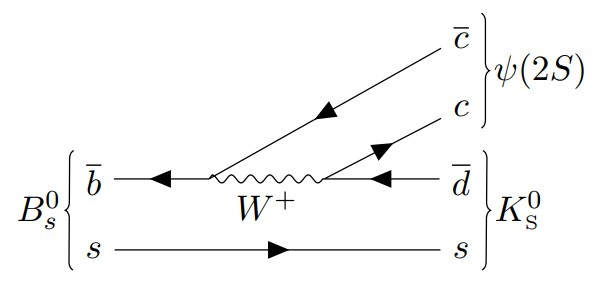
\includegraphics[width=0.5\linewidth]{Figure/decay.jpg}
    \caption{Leading order Feynman diagram of the decay $B_{s}^{0} \rightarrow \psi(2S)K_{s}^{0}$ in the Standard Model.}
    \label{decay}
\end{figure}

Three datasets are used for this analysis:\\
\begin{enumerate}
    \item The real data recorded by the LHCb experiment with a very rough
    selection.
    \item A sample of the signal decay $B_{s}^{0} \rightarrow \psi(2S)K_{s}^{0}$ obtained from Monte-Carlo simulation.
    \item A sample of the (kinematically) very similar decay $B^{0} \rightarrow \psi(2S)K_{s}^{0}$ obtained from Monte-Carlo simulation.
\end{enumerate}

The LHCb experiment uses an elaborate trigger system to select likely interesting events and
reduce the great amount of data to a size that is small enough to be stored. Often, the interesting events are are hidden in the real data sample
such that some further selection is required. In order to study the physics of $B_{s}^{0} \rightarrow \psi(2S)K_{s}^{0}$
events, a cleaner sample with
better signal to background ratio is required. Obtaining such a sample, using a multi-variate analysis (MVA)
to classify signal and background, is the aim of this study. A MVA classifier is a machine learning method used to distinguish between different categories or classes (e.g. signal vs. background) by analyzing multiple input variables simultaneously. The signal region should never be used in training the classifier to avoid bias. Otherwise, it might lead to false discovery.\\

Simulated data often differ from real data due to limitations in theoretical models and detector simulations. Improving accuracy would require significantly more computational resources, as simulating each event already takes several minutes and millions of events are needed per decay mode. To lower these discrepancies, kinematic weights are applied to simulation samples. These weights correct for differences between data and simulation in kinematic distributions, ensuring better alignment with real observations.\\

Since, the signal in the real dataset is hidden in the background, it is essential to use a loss function that needs to be minimized. The inverse of the loss function is called a figure of merit (FOM), which helps quantify the quality of a classifier. One important and common FOM in the high-energy physics (HEP) community is Punzi FOM \cite{punzi}. It is defined as:\\
\begin{align}
    FOM=\frac{\epsilon_{sig}}{\frac{5}{2}-\sqrt{N_{bkg}}}
\end{align}
where $N_{bkg}$ is the expected number of background events in the signal region and $\epsilon_{sig}$ is the classification efficiency of the signal. Again, $N_{bkg}$ can be defined as:\\
$$
    N_{bkg} = \text{No. of background events in the background region}\times\frac{\text{width of signal region}}{\text{width of background region}}.
$$

The background in the real dataset is mostly combinatorial. Combinatorial background consists of events that pass the selection purely due to coincidence. For example, two unrelated muons may accidentally appear to originate from a common vertex, prompting the reconstruction algorithm to falsely identify them as a $\psi(2S)$ candidate. If a nearby, randomly associated $K_{s}^{0}$ is also reconstructed, the algorithm may combine it with the $\psi(2S)$ to form a $B$ candidate. However, since the $\psi(2S)$ and 
$K_{s}^{0}$
  are uncorrelated in such cases, the resulting invariant mass of the reconstructed $B$ candidate can span a wide range. In contrast, true $B_{s}^{0} \rightarrow \psi(2S)K_{s}^{0}$
  decays will cluster around the nominal 
$B_{s}^{0}$
  mass, with well-defined kinematic and geometric properties. Because combinatorial background lacks such correlations, kinematic variables are particularly effective in distinguishing it from genuine signal events.\\
  
 In this experiment, there are a lot of instances where distributions will be compared. A trivial way to do that is to get the largest distance between the cumulative probability distributions(CDF). It can be defined as:\\
$$\sup_{n}\abs{{F_{n}^{1} - F_{n}^{2}}}$$
where n is the number of bins in the histogram. This can be easily obtained using the Kolmogorov-Smirnov (KS) test from the scipy package in coding \cite{ks}.\\

The final evaluation can be done using the significance which can be defined as:\\
\begin{align}
    m = \frac{N_{sig}}{\sqrt{N_{sig} + N_{bkg}}}
    \label{proxy}
\end{align}

where $N_{bkg}$ is the number of background candidates and $N_{sig}$ is the number of signal candidates. This significance is a measure of how likely the result is produced by statistical calculations. A discovery is claimed if the significance is greater than 5. If the significance is larger than 3, then there is evidence of the signal.\\
\chapter{Dataset Description}\label{ch2}
Table \ref{tab:data_sim_samples} summarizes the datasets and simulated samples used in this analysis. It includes the recorded proton-proton collision data from 2016 as well as various Monte Carlo simulated backgrounds and signal samples.

\renewcommand{\arraystretch}{1.3} % increase row height
\begin{table}[h!]
\centering
\caption{pp collisions recorded in 2016 at \(\sqrt{s} = 13\) TeV}
\label{tab:data_sim_samples}
\begin{tabular}{@{}l p{8cm}@{}}
\toprule
\textbf{Sample} & \textbf{Description} \\ \midrule
Data & Events selected with a single-lepton trigger: electrons with \(E_T > 25\) GeV or muons with \(p_T > 25\) GeV. \\[6pt]

SM \(t\bar{t}\) background & Simulated at next-to-leading order (NLO) with parton shower. \\
                           % & Scaled to next-to-next-to-leading order (NNLO) + next-to-next-to-leading logarithmic (NNLL) cross sections. \\[6pt]

Other backgrounds & Single-top events using best available theoretical predictions. \\
                       & \(W\)+jets and \(Z\)+jets events \\
                       % , scaled using best available theoretical predictions. 
                       % & Diboson (\(WW\), \(WZ\), \(ZZ\)) events\\ , scaled using best available theoretical predictions. \\[6pt]

\(Z'\) signal & \\ 
Mass points: 500–3000 GeV & Narrow width assumption \((\Gamma / m \approx 1\%)\). \\
                       & SM-like coupling to \(t\bar{t}\) with full detector simulation. \\
\bottomrule
\end{tabular}
\end{table}









\chapter{Results and Analysis}

The invariant mass distribution of the real data is shown in Figure \ref{inv_mass_data}. For simplicity, it was assumed that the invariant mass distribution shown in the figure is composed only of the decays originating from the signal and control channels and from the combinatorial background. The peak in Figure \ref{inv_mass_data} is caused by $B^{0} \rightarrow \psi(2S)K_{s}^{0}$ decays, while the signal decay ($B_{s}^{0} \rightarrow \psi(2S)K_{s}^{0}$) cannot be observed as it is submerged by combinatorial background.\\   
    \begin{figure}[H]
        \centering
        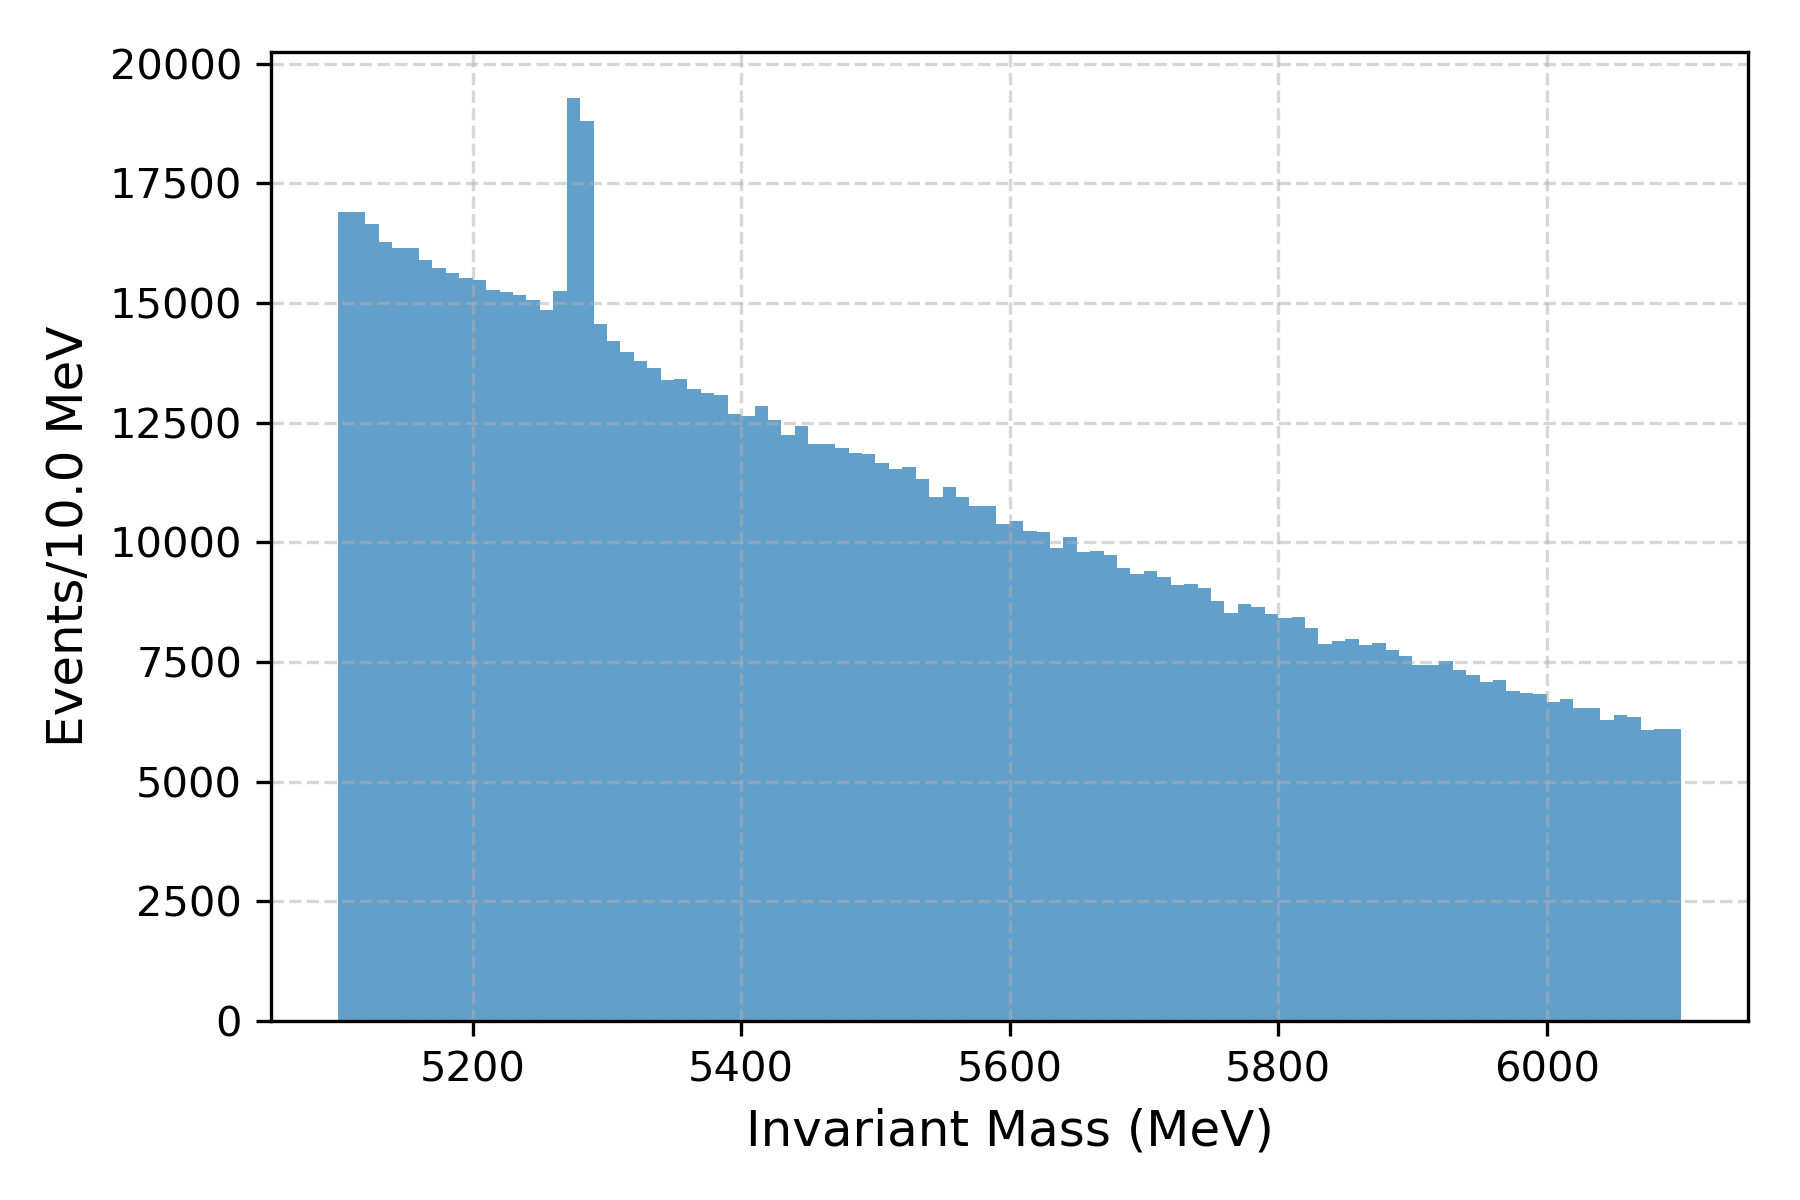
\includegraphics[width=0.7\linewidth]{Figure/2_data_invariant_mass_distribution.png}
        \caption{Reconstructed invariant mass distribution of the real data set.}
        \label{inv_mass_data}
    \end{figure}

    \section{Signal Region and Background Sample}
    In order to define the signal region in the real dataset, a selection was made in the real dataset was made with the help of the signal simulation dataset. First, a window containing $99\%$ of the data was found in the signal dataset as shown Figure \ref{in_mass_sig}.\\

    \begin{figure}[H]
        \centering
        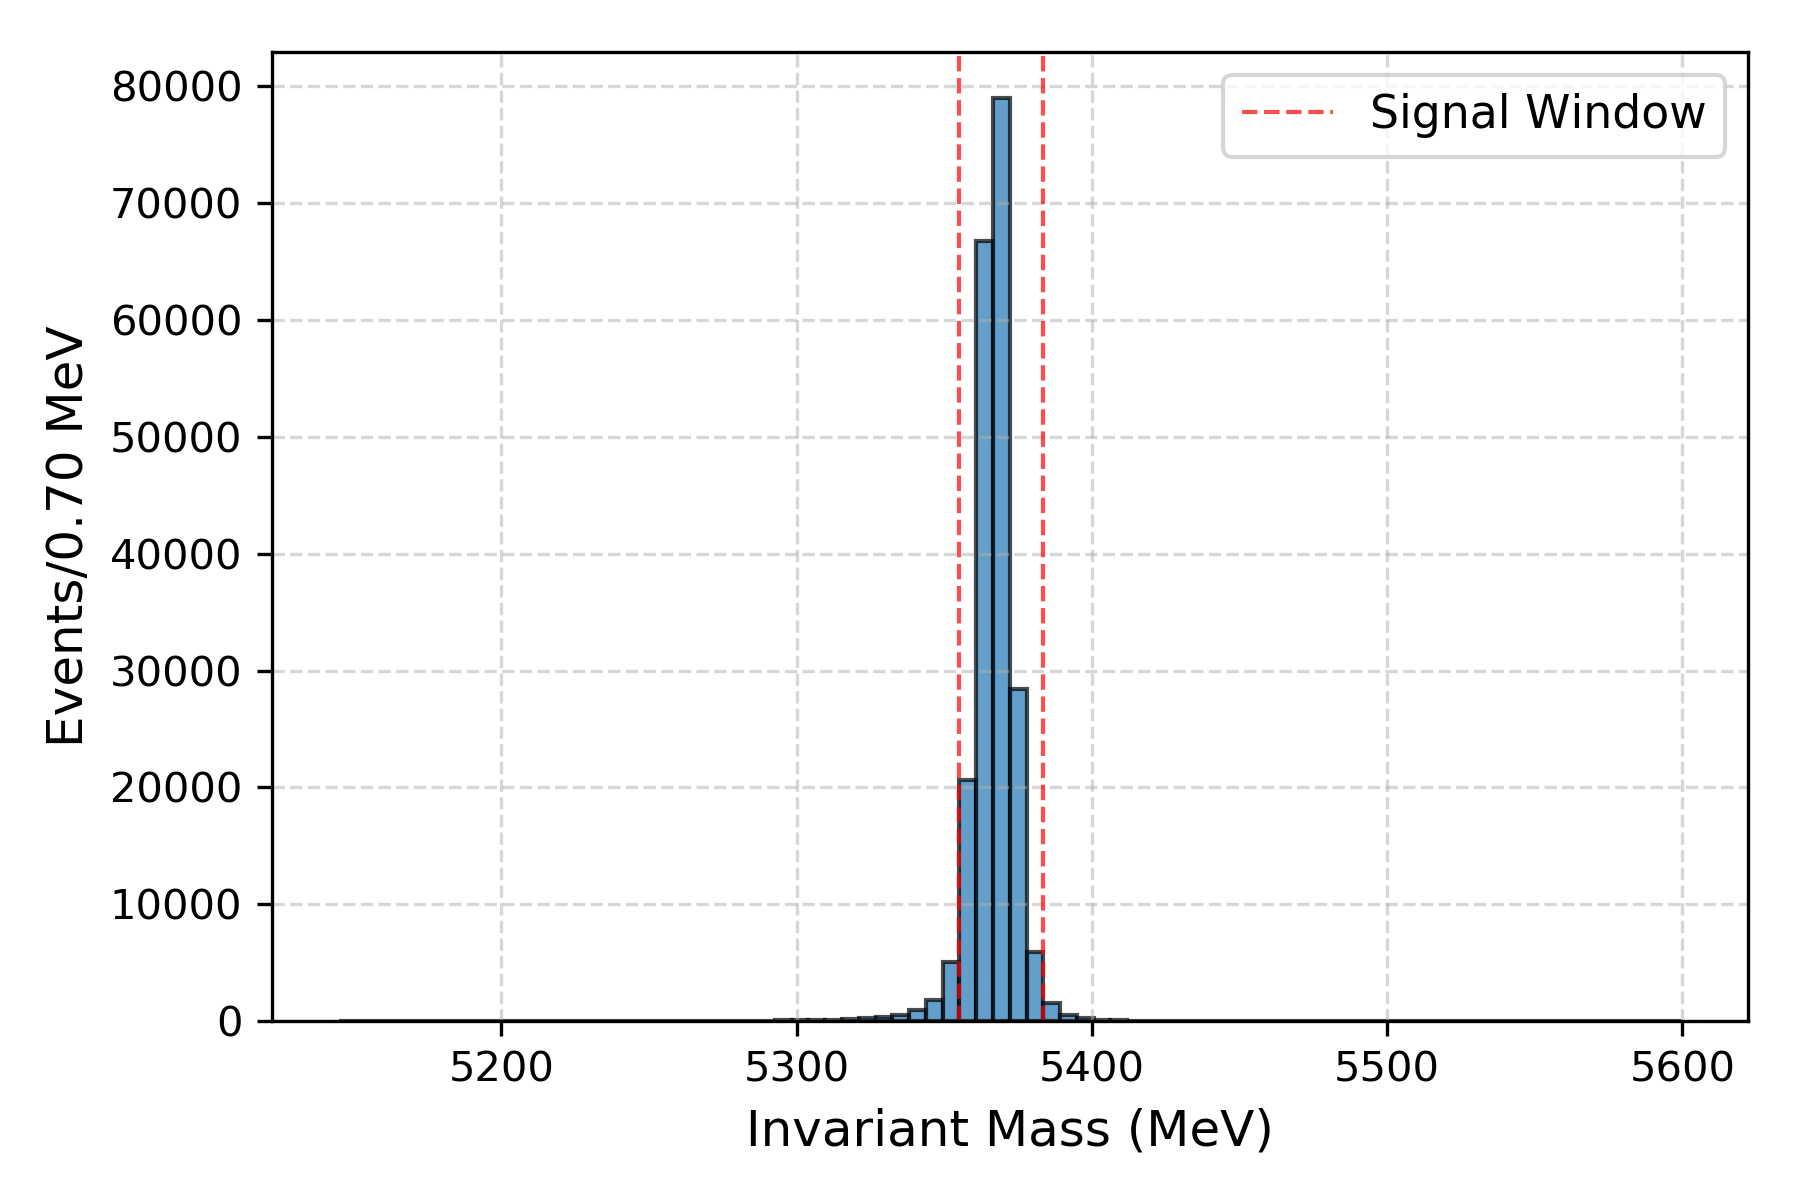
\includegraphics[width=0.7\linewidth]{Figure/3_signal_invariant_mass_distribution_99_data.png}
        \caption{Reconstructed invariant mass distribution of the signal simulation.}
        \label{in_mass_sig}
    \end{figure}
    Afterwards, this window is implemented in the invariant mass distribution of the real dataset as shown in Figure \ref{inv_mass_data_99}\\
    \begin{figure}[H]
        \centering
        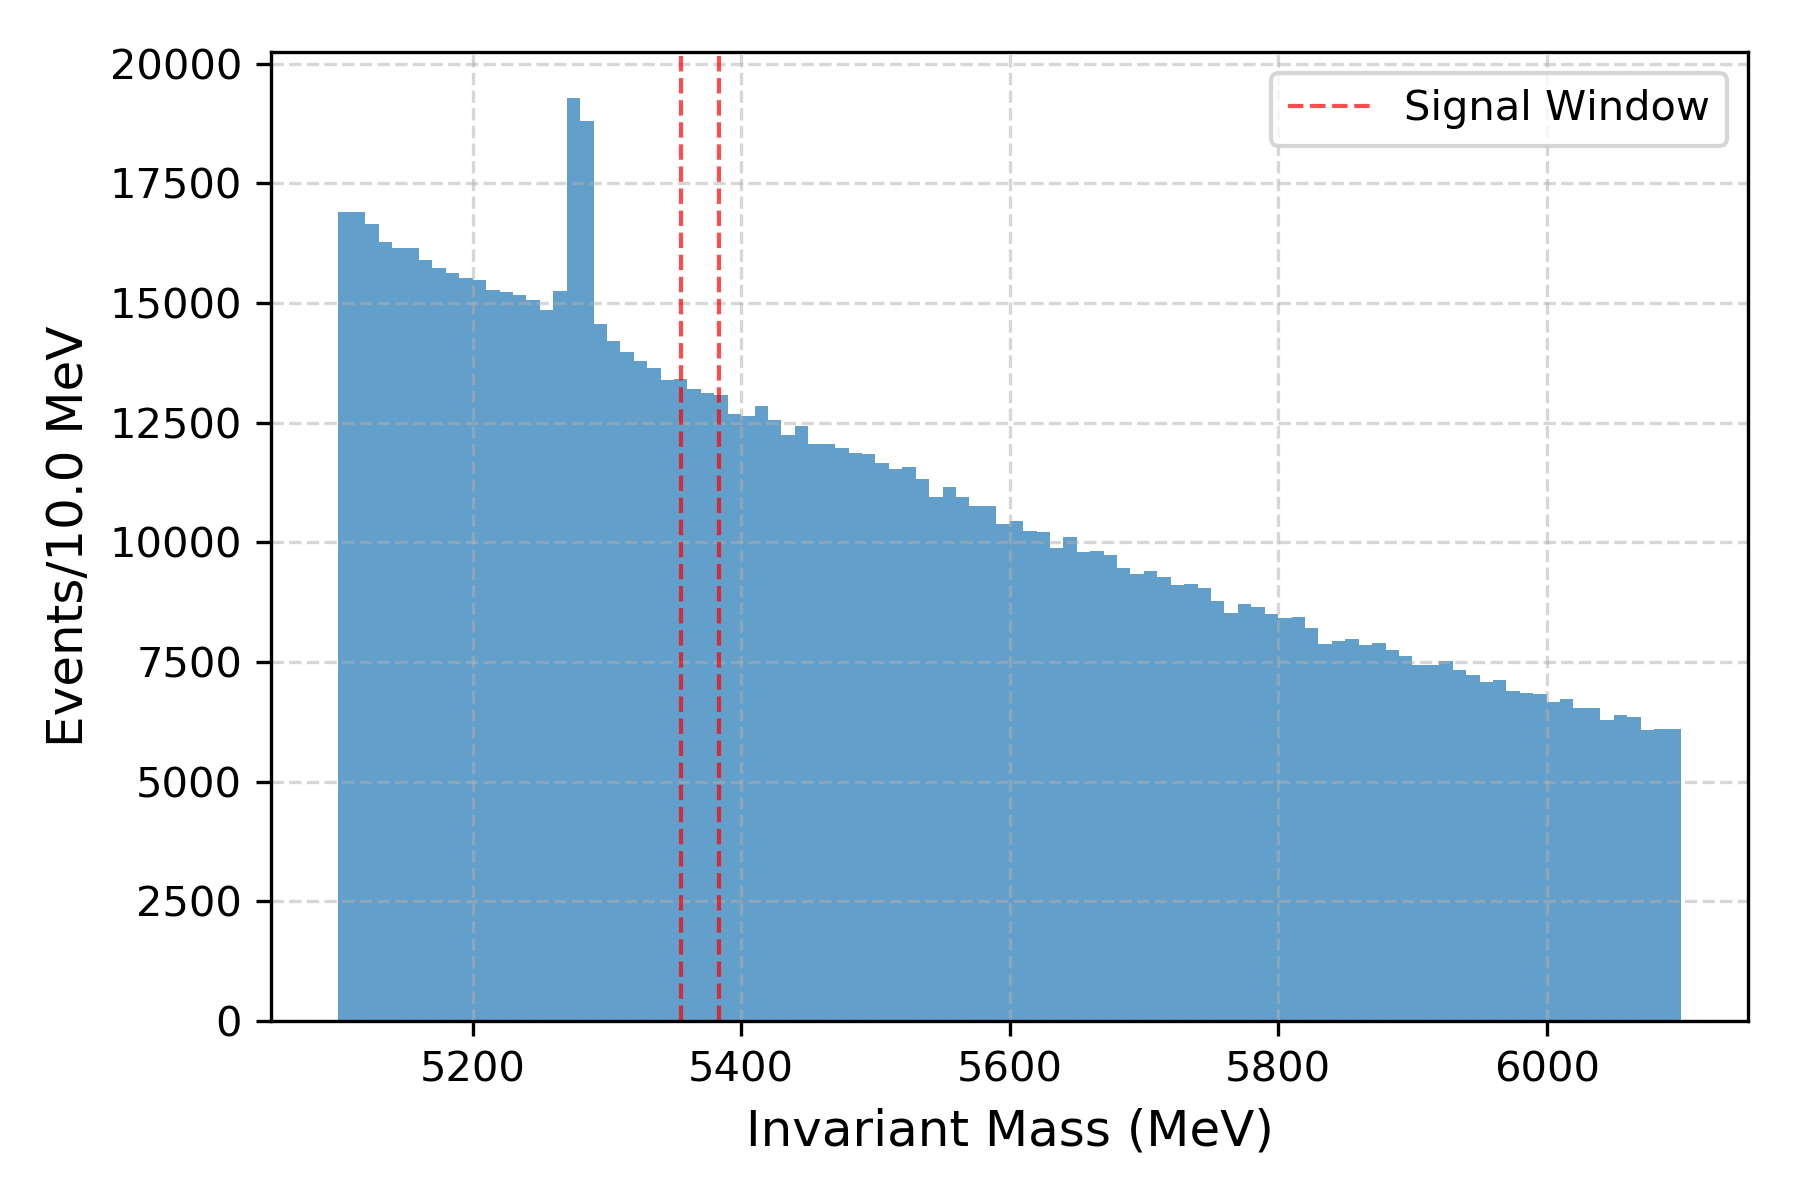
\includegraphics[width=0.7\linewidth]{Figure/4_data_invariant_mass_distribution.png}
        \caption{Implemented signal region in the real data set invariant mass distribution.}
        \label{inv_mass_data_99}
    \end{figure}
    
    The two Monte Carlo simulations do not contain any background, so the background must be identified within the real data set. So, to train the MVA to recognize background, background from the real data sample shall be used. Hence, the upper side band (USB) of the real data set was taken as the background sample, i.e. all the data in the real data set that have invariant mass higher than the right side of the signal region. The signal simulation dataset and the background candidates obtained from the USB are used for the MVA training.\\

    In the real data set, there is a column with weights, which if used gives the pure $B^{0}$ events. The figure below shows the distribution with and without these weights.\\ 
    
    \begin{figure}[H]
        \centering
        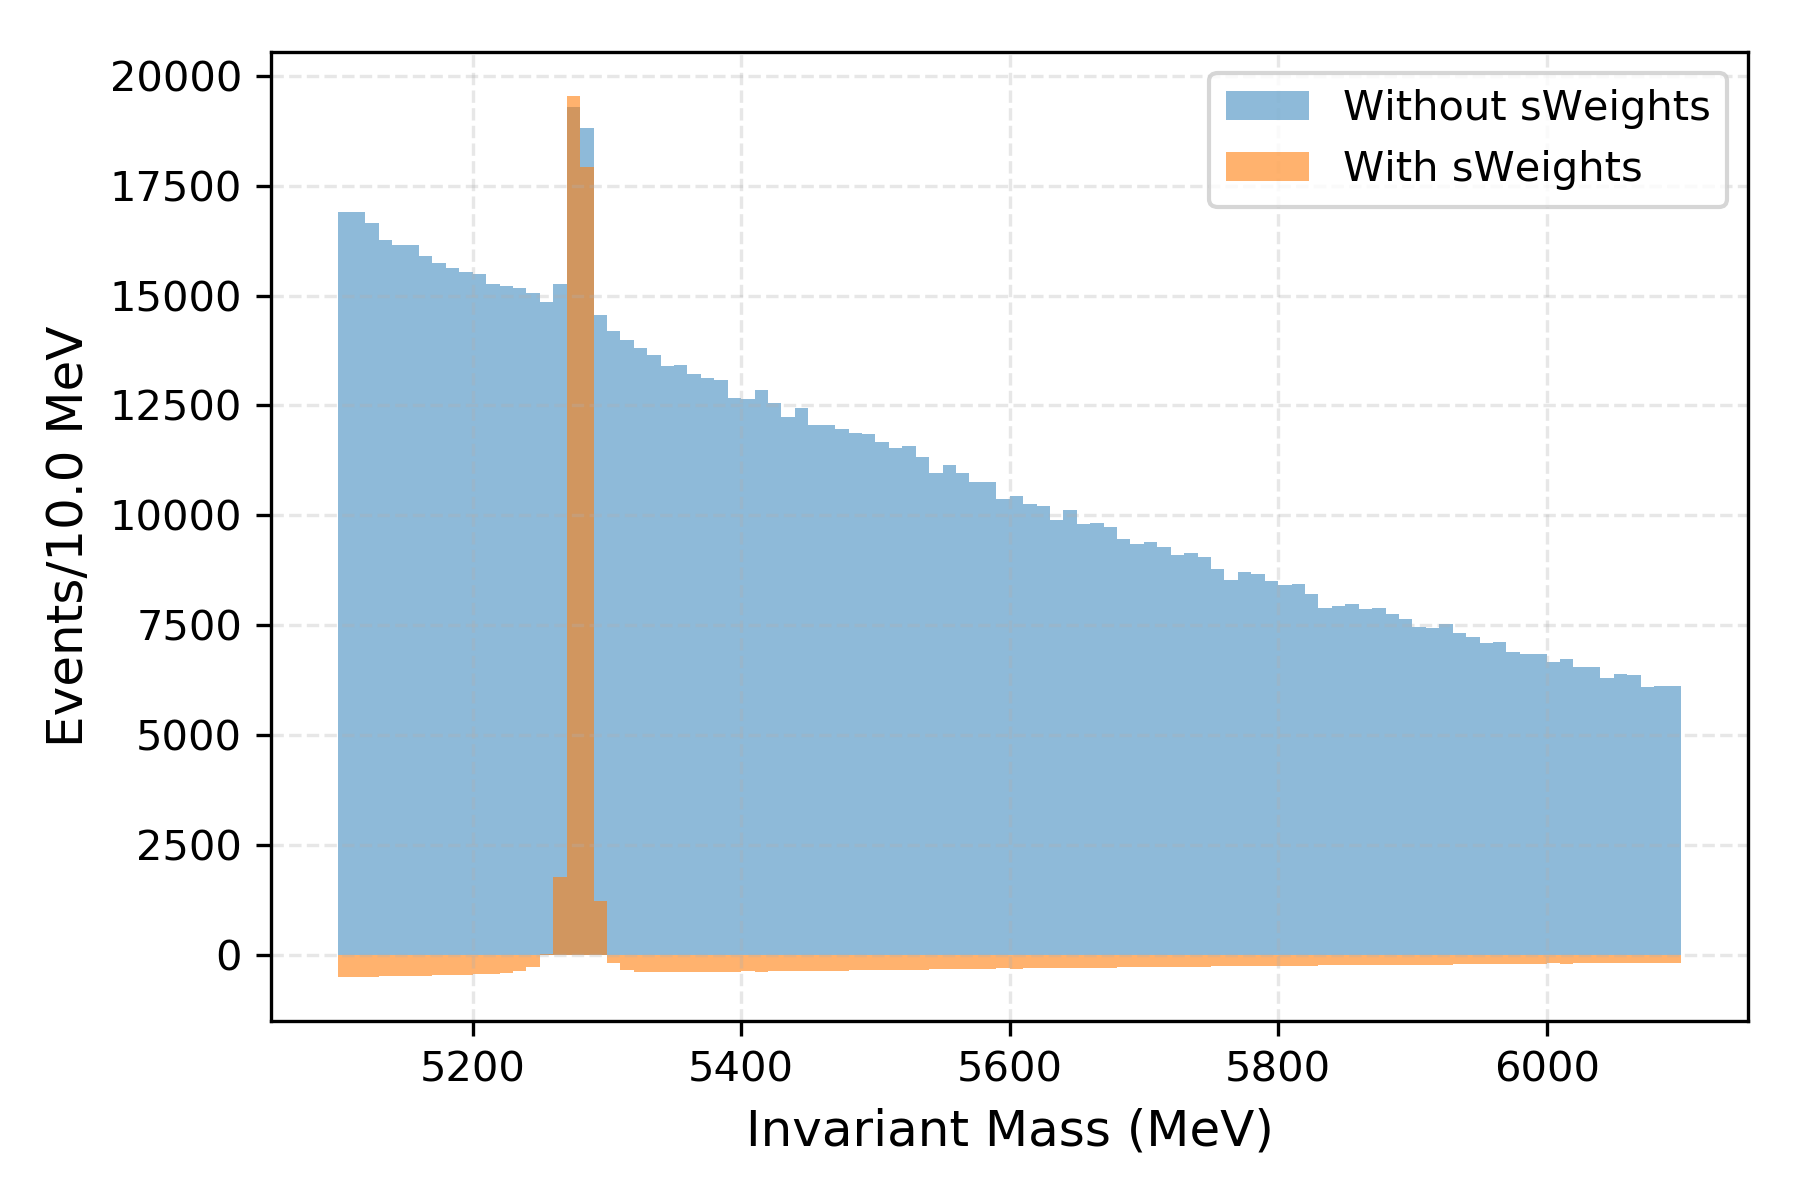
\includegraphics[width=0.7\linewidth]
        {Figure/5_data_invariant_mass_distribution_sWeights.png}
        \caption{Invariant mass distribution as returned by the trigger line (blue) and invariant mass distribution of the $B^{0}$ candidates, highlighted using background subtraction (s-weights) whights (orange).}
        \label{pure}
    \end{figure}

%$B_{s}^{0} \rightarrow \psi(2S)K_{s}^{0}$
    
    \section{Feature Selection}
    Even after using the weights there are many differences in the distribution due to various reasons. A large number of features will make the model slow and also lead to overfitting whereas a small amount of features will make poor predictions. Not all of the features in the dataset contain useful information. In order to select suitable features, the KS test was used.\\
    
    Hence, features which satisfies the following conditions must be used for training the model:
    \begin{enumerate}
        \item Reasonable agreement between data and simulation (otherwise the classifier only learns to distinguish data from simulation instead of signal from background).
        \item Strong discrimination between signal (simulation) and background (USB).
        \item Uncorrelated to the invariant mass of the $B_{s}^{0}/B^{0}$
      candidate.
    \end{enumerate}
    Using the KS test, 27 suitable features were found based on the above criteria. In order to find similarity between the $B^{0}$ simulation and $B^{0}$ data, a threshold KS < 0.05 had been used and to distinguish between the signal and the background a threshold of KS > 0.2 had been used. In this test, the KS metric had values [0, 1] where 0 means that the distributions are identical and 1 means that the distributions are completely different. The thresholds used in the analysis are achieved via exploratory analysis.

    \section{Training the Classifier and Optimization}
    The machine learning model used in the analysis was XGBClassifier, which is a supervised learning model. Since, the number of background data is very large compared to the number of signal data, weights has been used to make accurate predictions. Because, imbalanced data can lead to misleading or biased classifications. Afterwards, hyperparameter optimization was done to slightly improve the performance of the model. In this case, RandomizedSearchCV, which is a hyperparameter tuning technique provided by scikit-learn library, had been used. The best parameters obtained from the optimizations are shown in Table \ref{hyperparameter}.\\
    
\begin{table}[H]
        \centering
        \begin{tabular}{cc}
            \hline
            Parameters & Best Values\\
            \hline
             \texttt{n\_estimators} & $1000$ \\
             \texttt{max\_depth} & $6$ \\
             \texttt{learning\_rate} &  $0.1$ \\
             \texttt{lambda} & $1$ \\
             \hline
        \end{tabular}
        \caption{Best parameters obtained from hyperparameter optimization.}
        \label{hyperparameter}
    \end{table}
    
    The evaluation of the model can be done with the following receiver operating characteristic (ROC) curve and confusion matrix.\\

    \begin{figure}[H]
        \centering
        \begin{subfigure}[b]{0.49\linewidth}
            \centering
            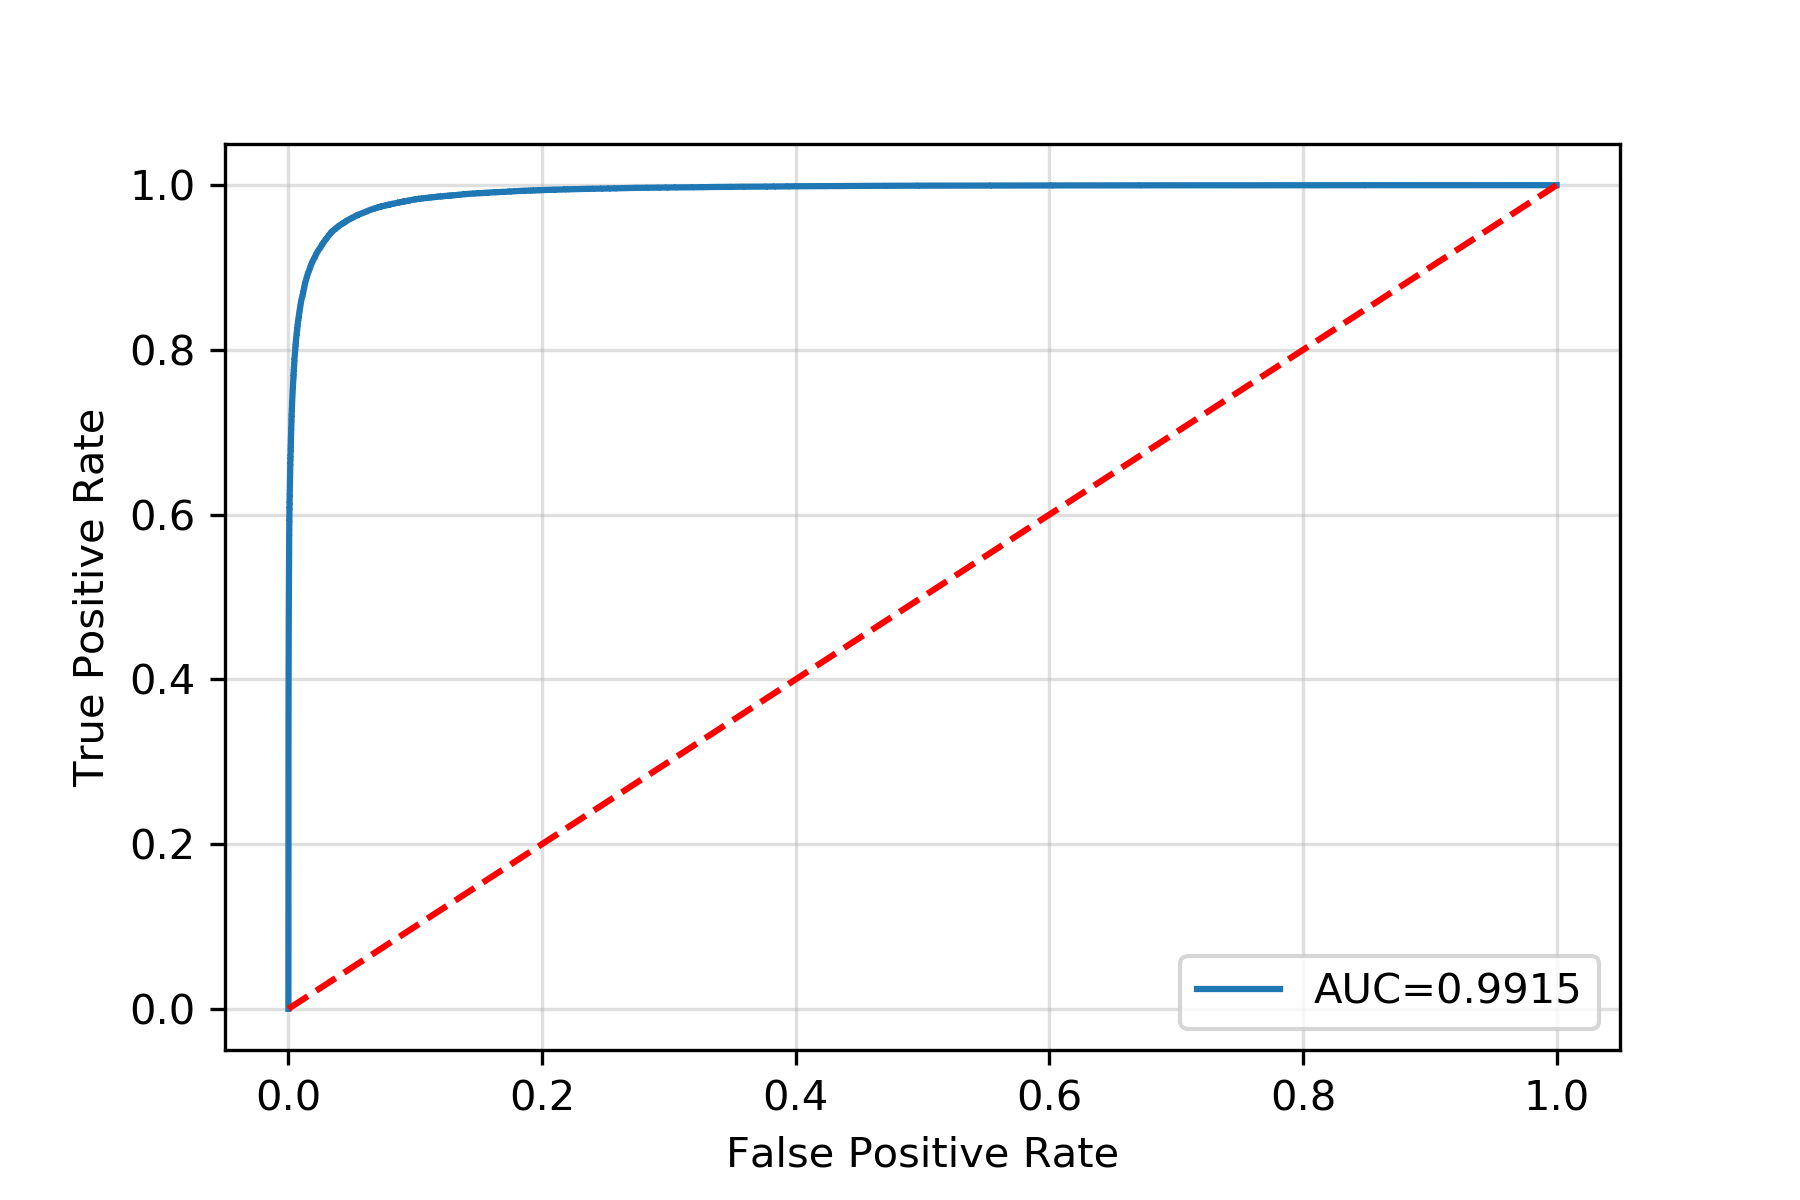
\includegraphics[width=0.95\linewidth]{Figure/roc_curve.png}
            \caption{ROC curve with the total area under the curve (AUC) value.}
            \label{roc_curve}
        \end{subfigure}
        \hfill
        \begin{subfigure}[b]{0.49\linewidth}
            \centering
            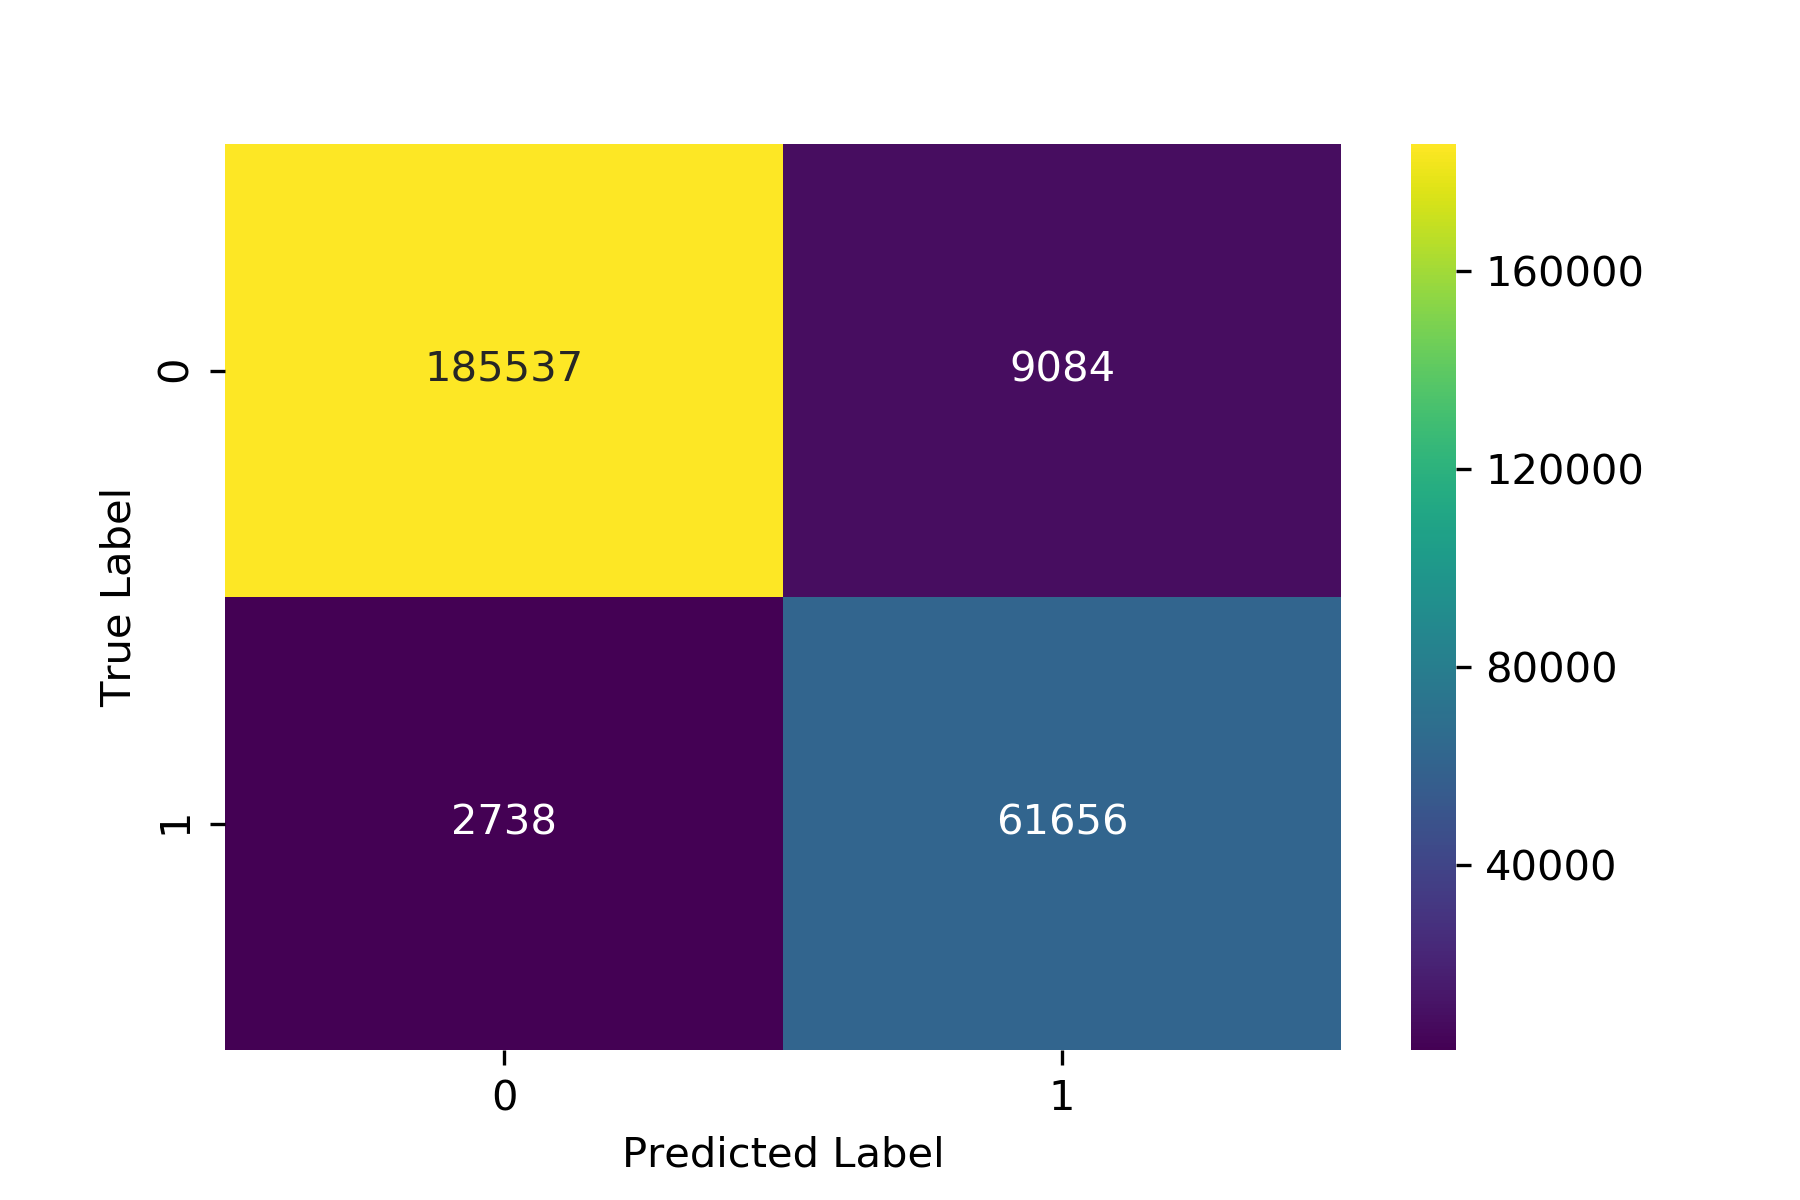
\includegraphics[width=0.95\linewidth]{Figure/confusion_matrix.png}
            \caption{Confusion matrix.}
            \label{confusion_matrix}
        \end{subfigure}
        \caption{Evaluation of the BDT model.}
    \end{figure}
    Both the confusion matrix and AUC score suggest that the model was trained well. The AUC score is especially useful in this scenario, when the dataset is heavily dominated by background samples. Another parameter is the boosted decision tree (BDT) score, which is a numeric output of a boosted decision tree classifier such as XGBClassifier, that reflects how strongly the model classifies a given event as signal or background. The distribution of the BDT score is shown in Figure \ref{dist}.\\
    
    \begin{figure}[H]
        \centering
        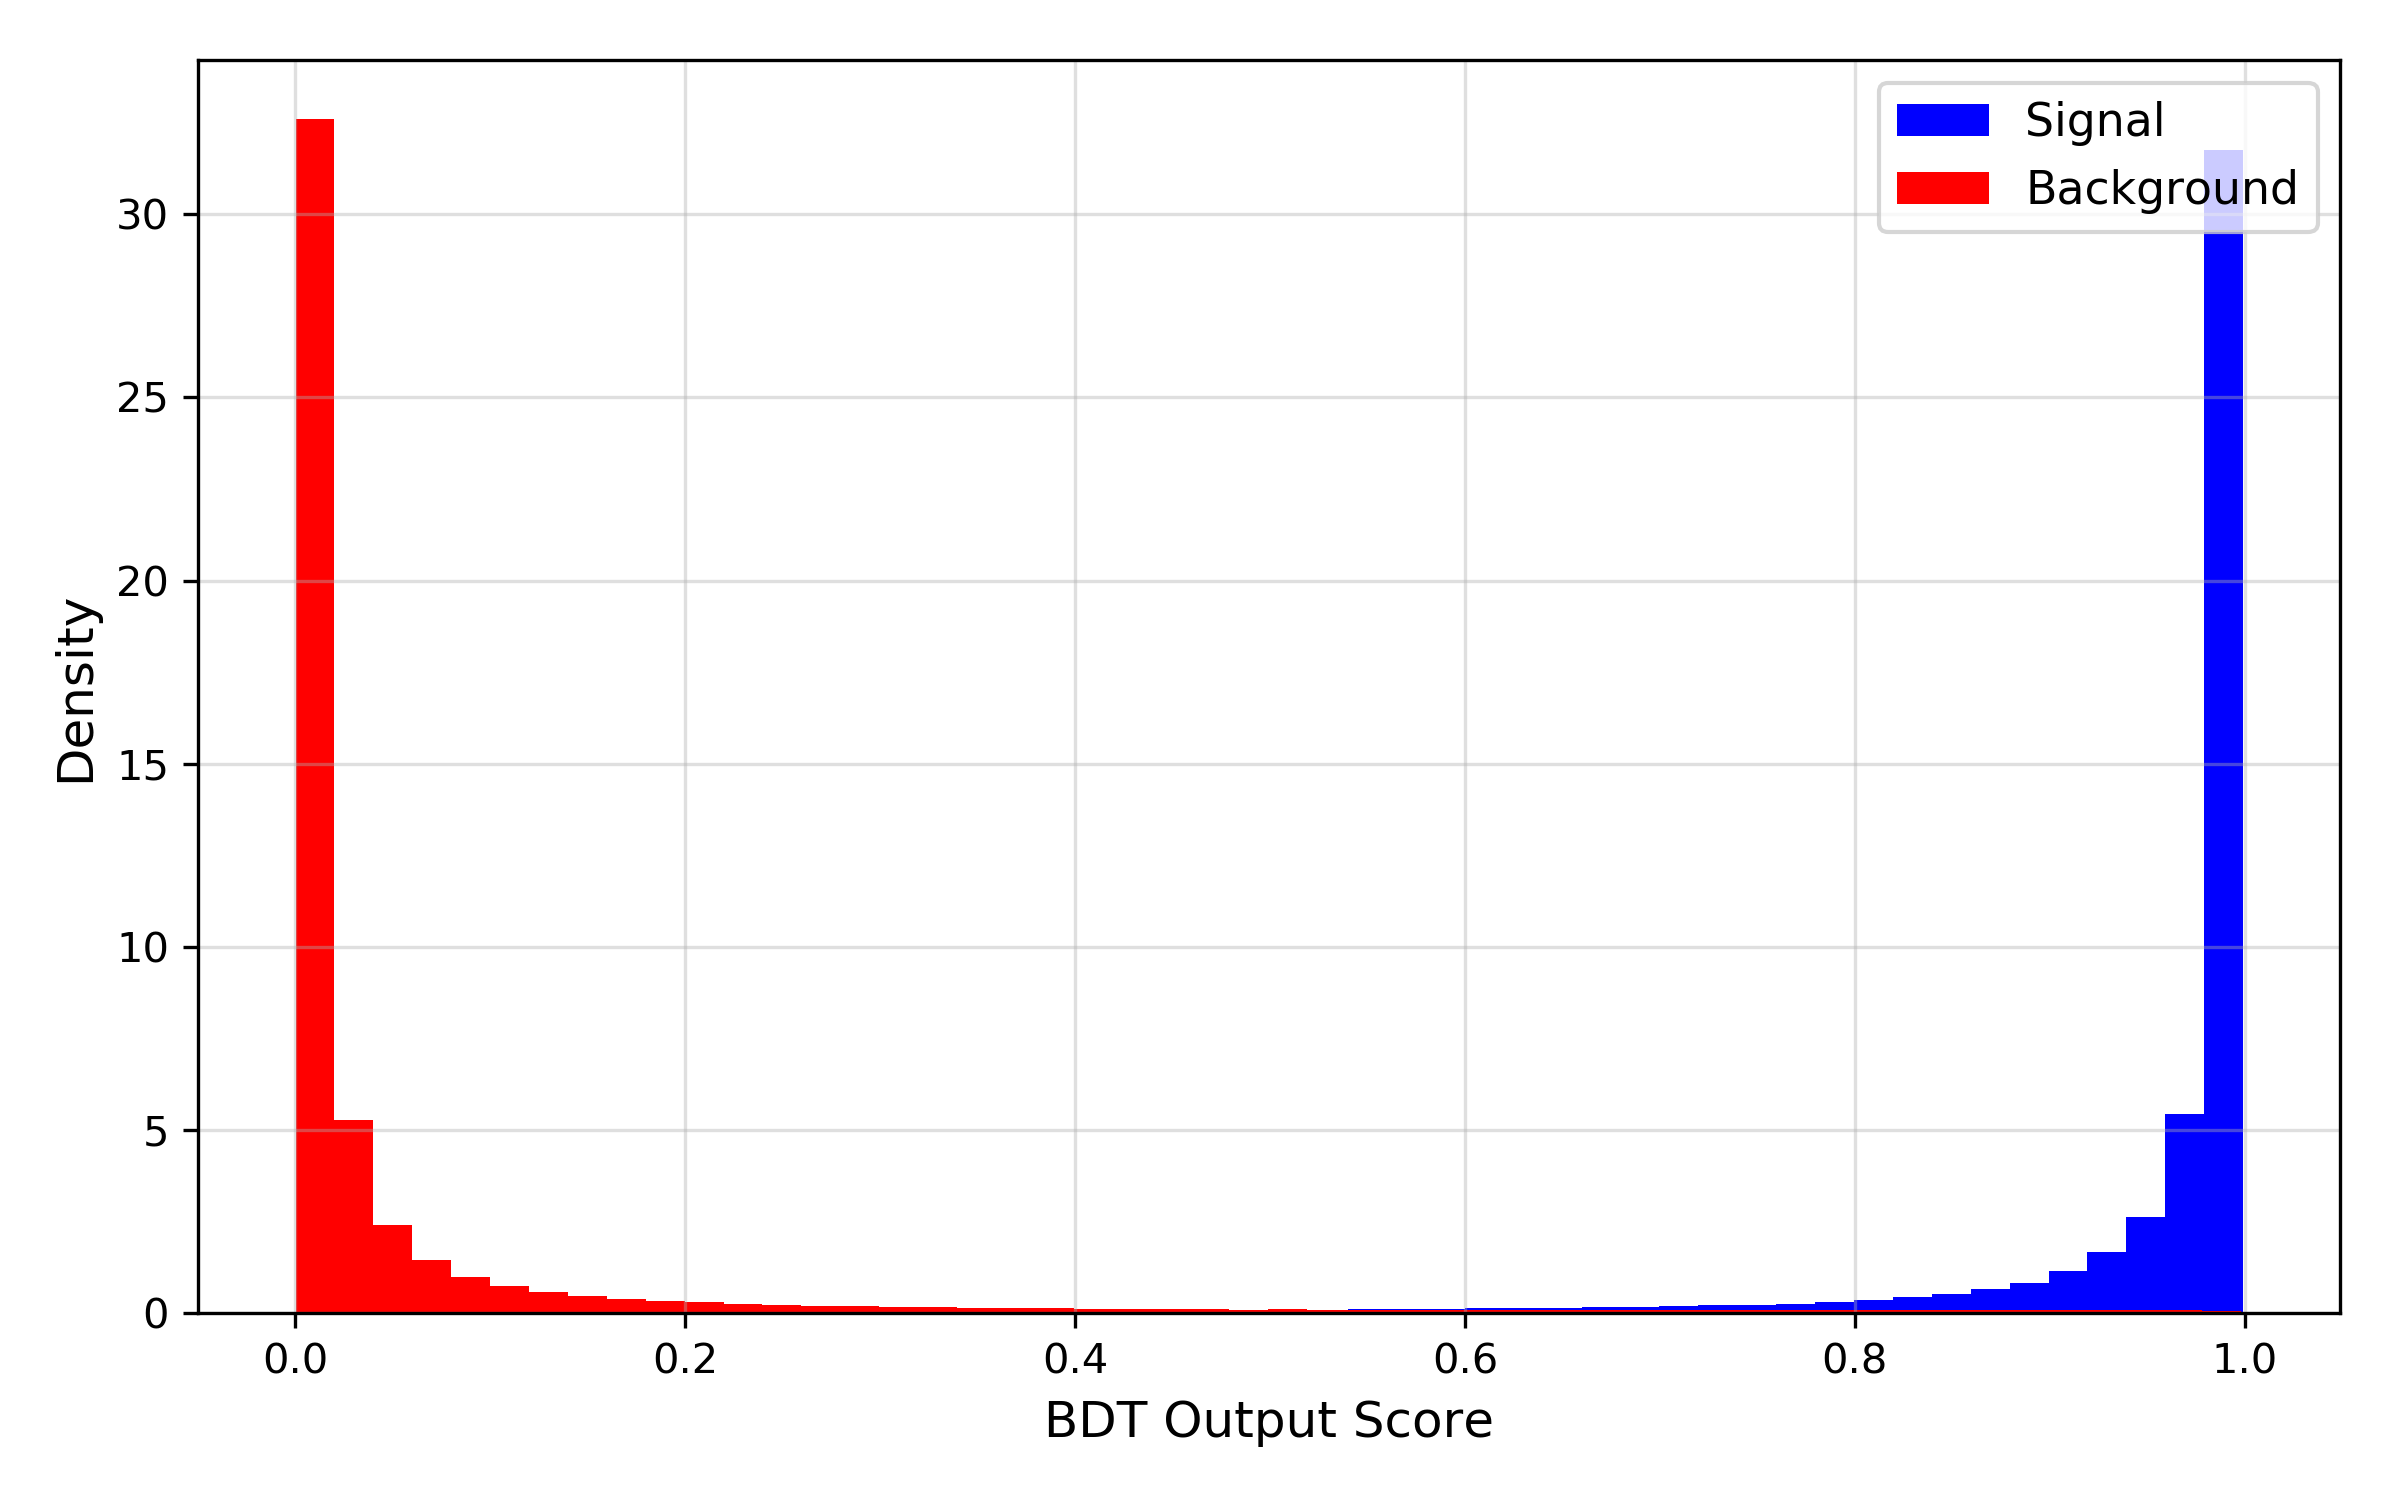
\includegraphics[width=0.7\linewidth]{Figure/6_BDT_Score.png}
        \caption{Distribution of the BDT output for background and signal samples.}
        \label{dist}
    \end{figure}

    From Figure \ref{sig_vs_thres}, it can be easily found that the best cut value which maximizes the Punzi FOM is $0.9919$. A plot of significances vs. threshold is shown in Figure \ref{sig_vs_thres}.

    \begin{figure}[H]
        \centering
        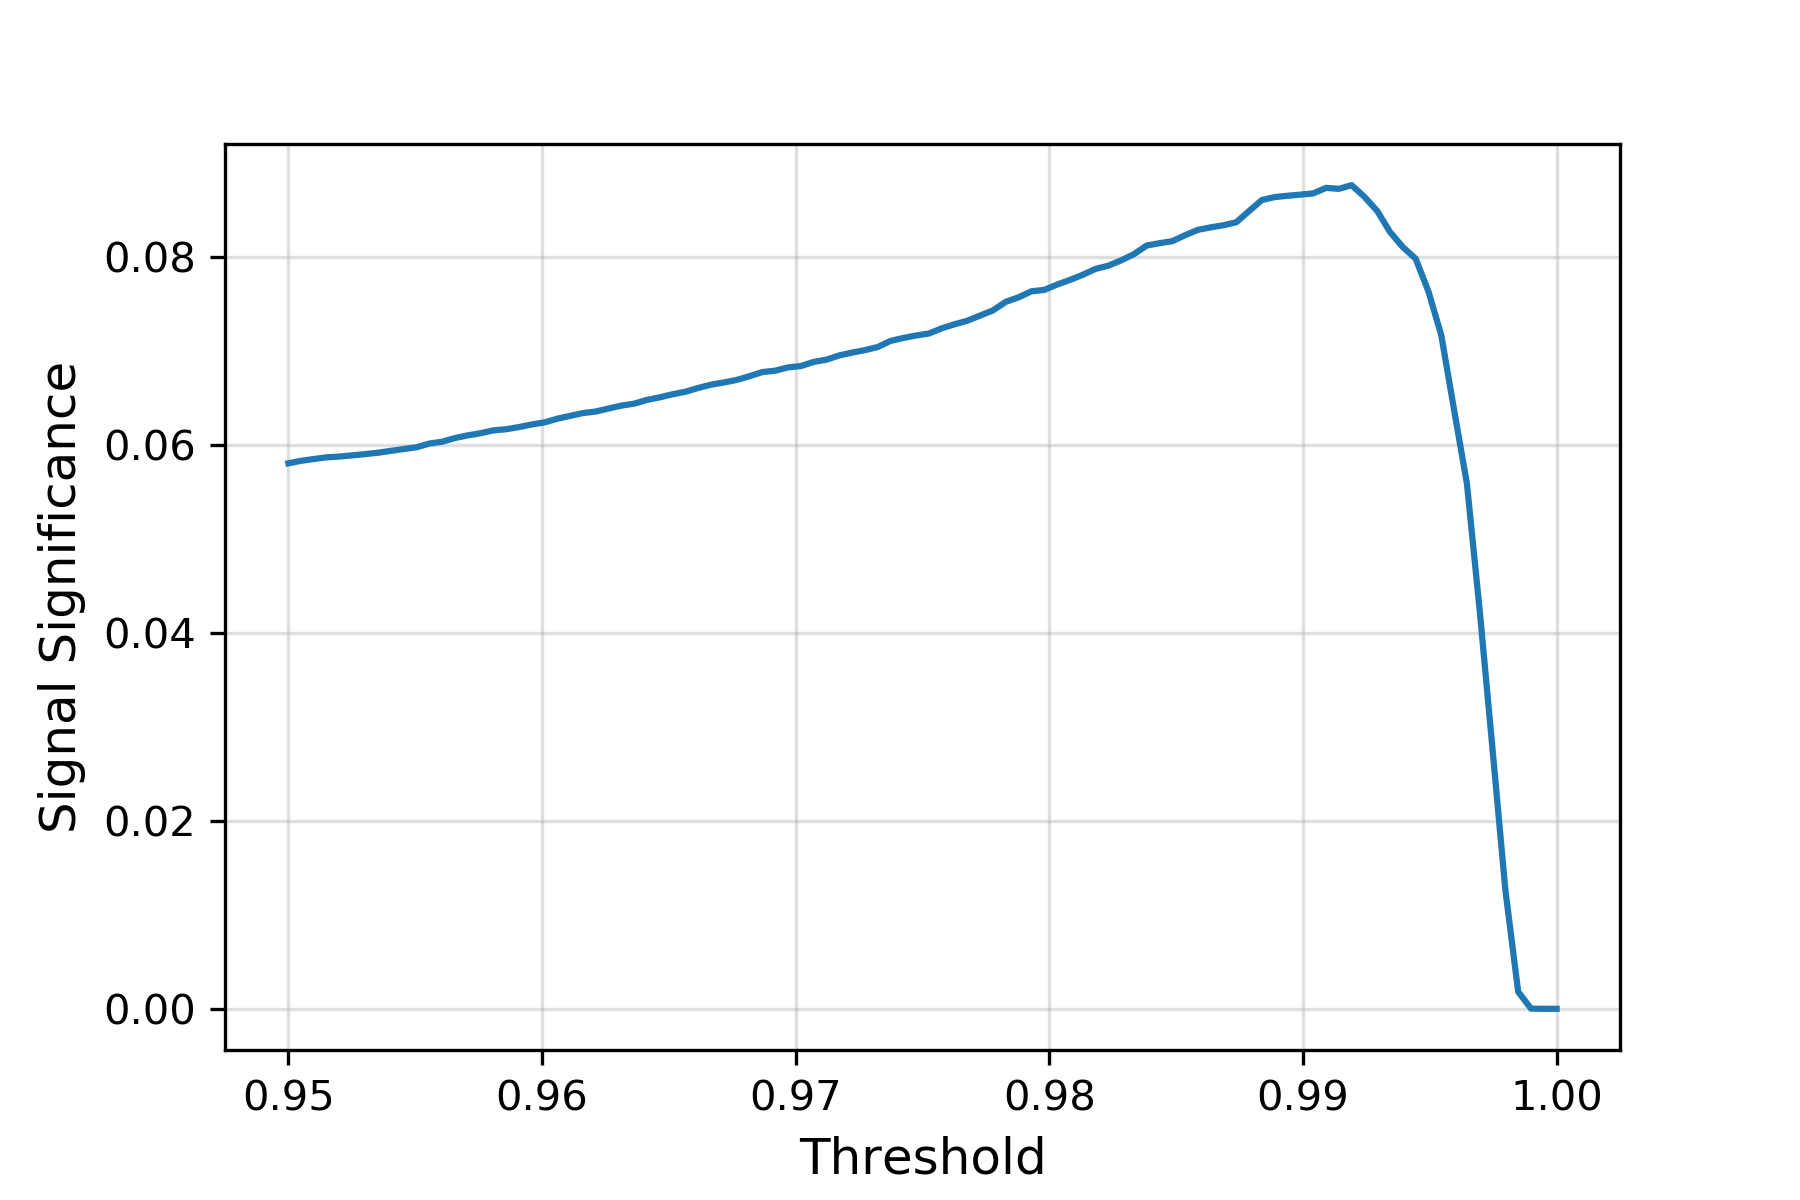
\includegraphics[width=0.5\linewidth]{Figure/7_significance_vs_threshold.png}
        \caption{Plot of Punzi FOM as a function of threshold.}
        \label{sig_vs_thres}
    \end{figure}
    Applying this best cut, a purer plot of the real data sample can be obtained as shown in Figure \ref{last_inv}.\\
    \begin{figure}[H]
        \centering
        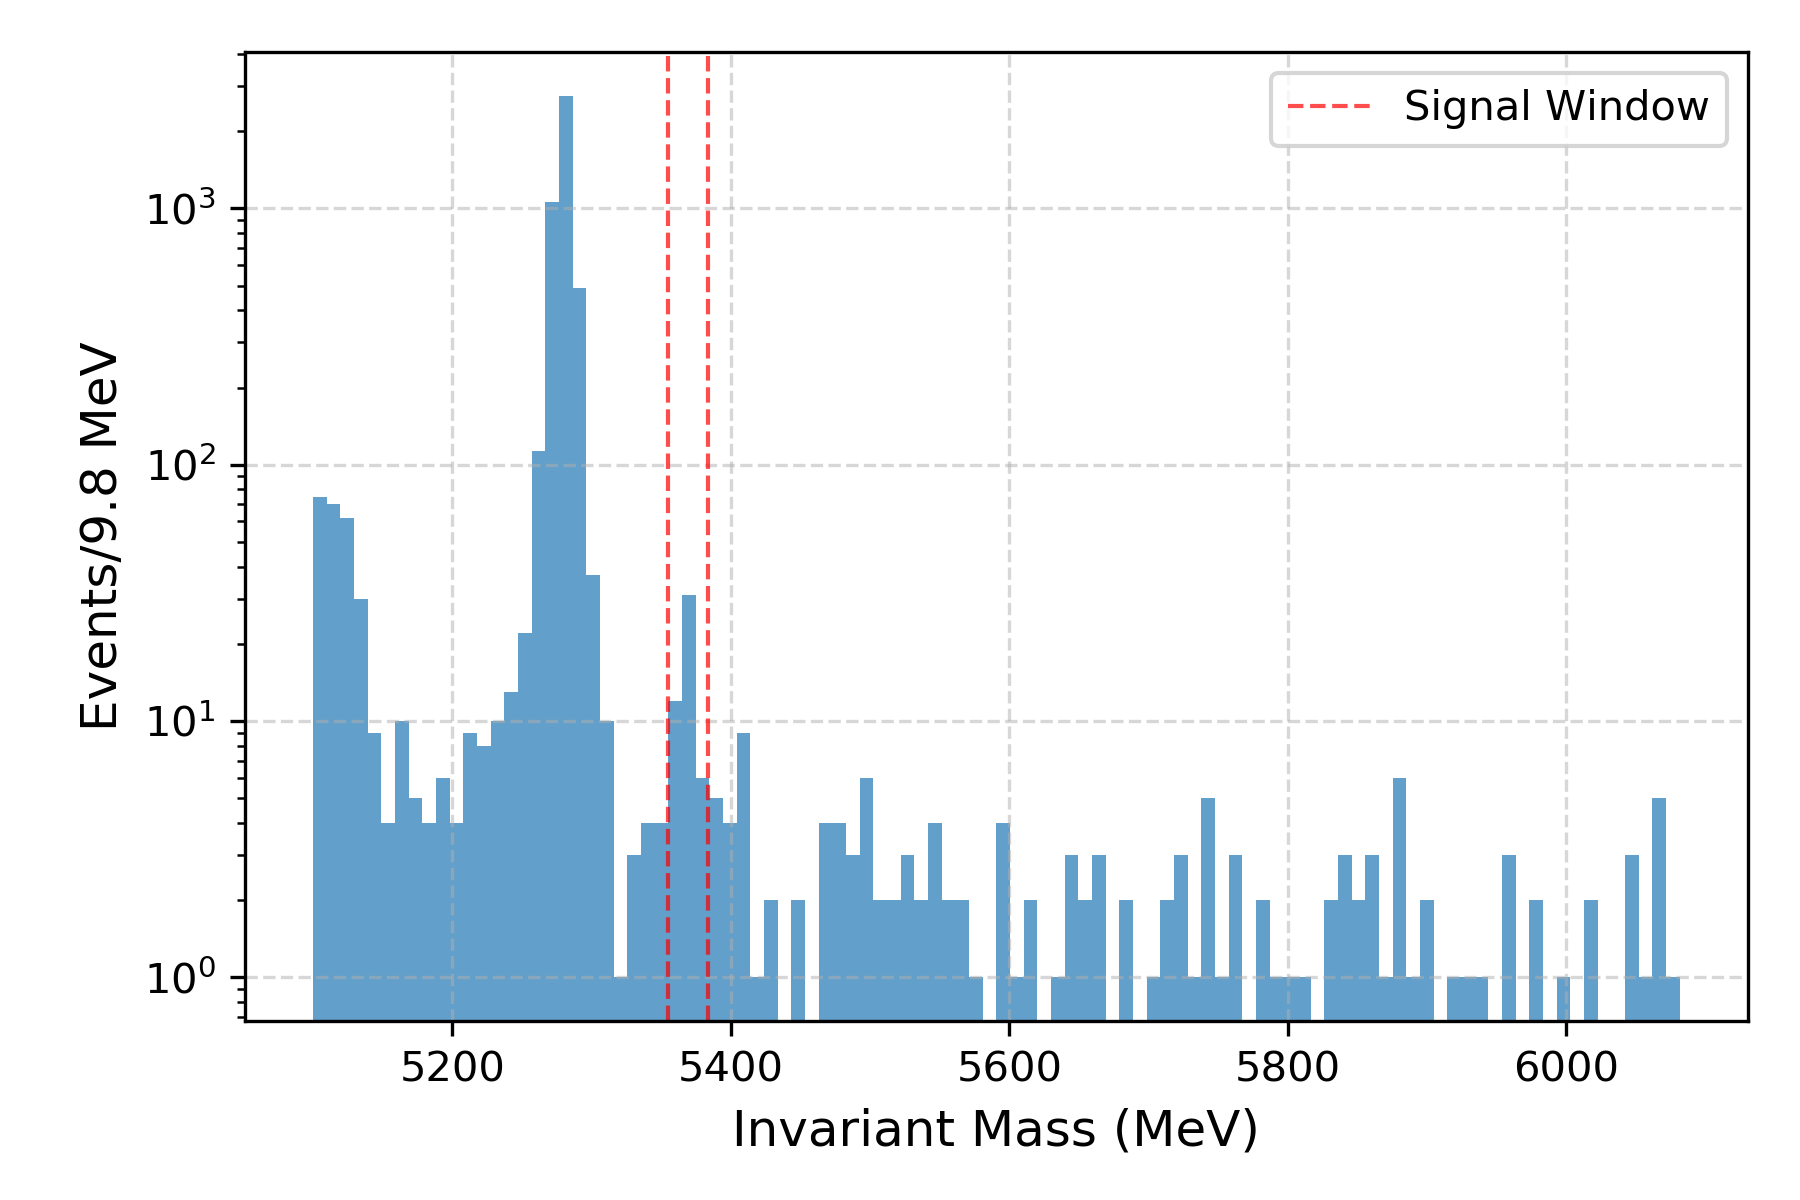
\includegraphics[width=0.5\linewidth]{Figure/8_data_invariant_mass_distribution.png}
        \caption{Selected mass distribution of the real data set.}
        \label{last_inv}
    \end{figure}
    In Figure \ref{last_inv}, two peaky structures can be observed in the regions where we expect the  $B_{s}$ and $B^{0}$ mass peaks.

    \section{Finding the Signal in the Data Sample}
    If peaks are fitted in the signal and control simulation using Gaussian function, then Figure \ref{fit_signal_peak} and \ref{fit_control_peak} are obtained. A Gaussian function has been used to fit peaks in signal and control simulations because it models the symmetric distribution of reconstructed quantities around their true values due to detector resolution, which provides with simple and symmetric signal shape. The formula for a Gaussian function (also known as the normal distribution) is:\\

    \begin{align}
        f(x) = A \cdot e^{-\frac{(x - \mu)^2}{2\sigma^2}}
    \end{align}
    where A is the height of the peak (amplitude), $\mu$ is the mean, $\sigma$ is the standard deviation and $e$ is the Euler's number.\\
    \begin{figure}[H]
        \centering
        \begin{subfigure}[b]{0.49\linewidth}
            \centering
            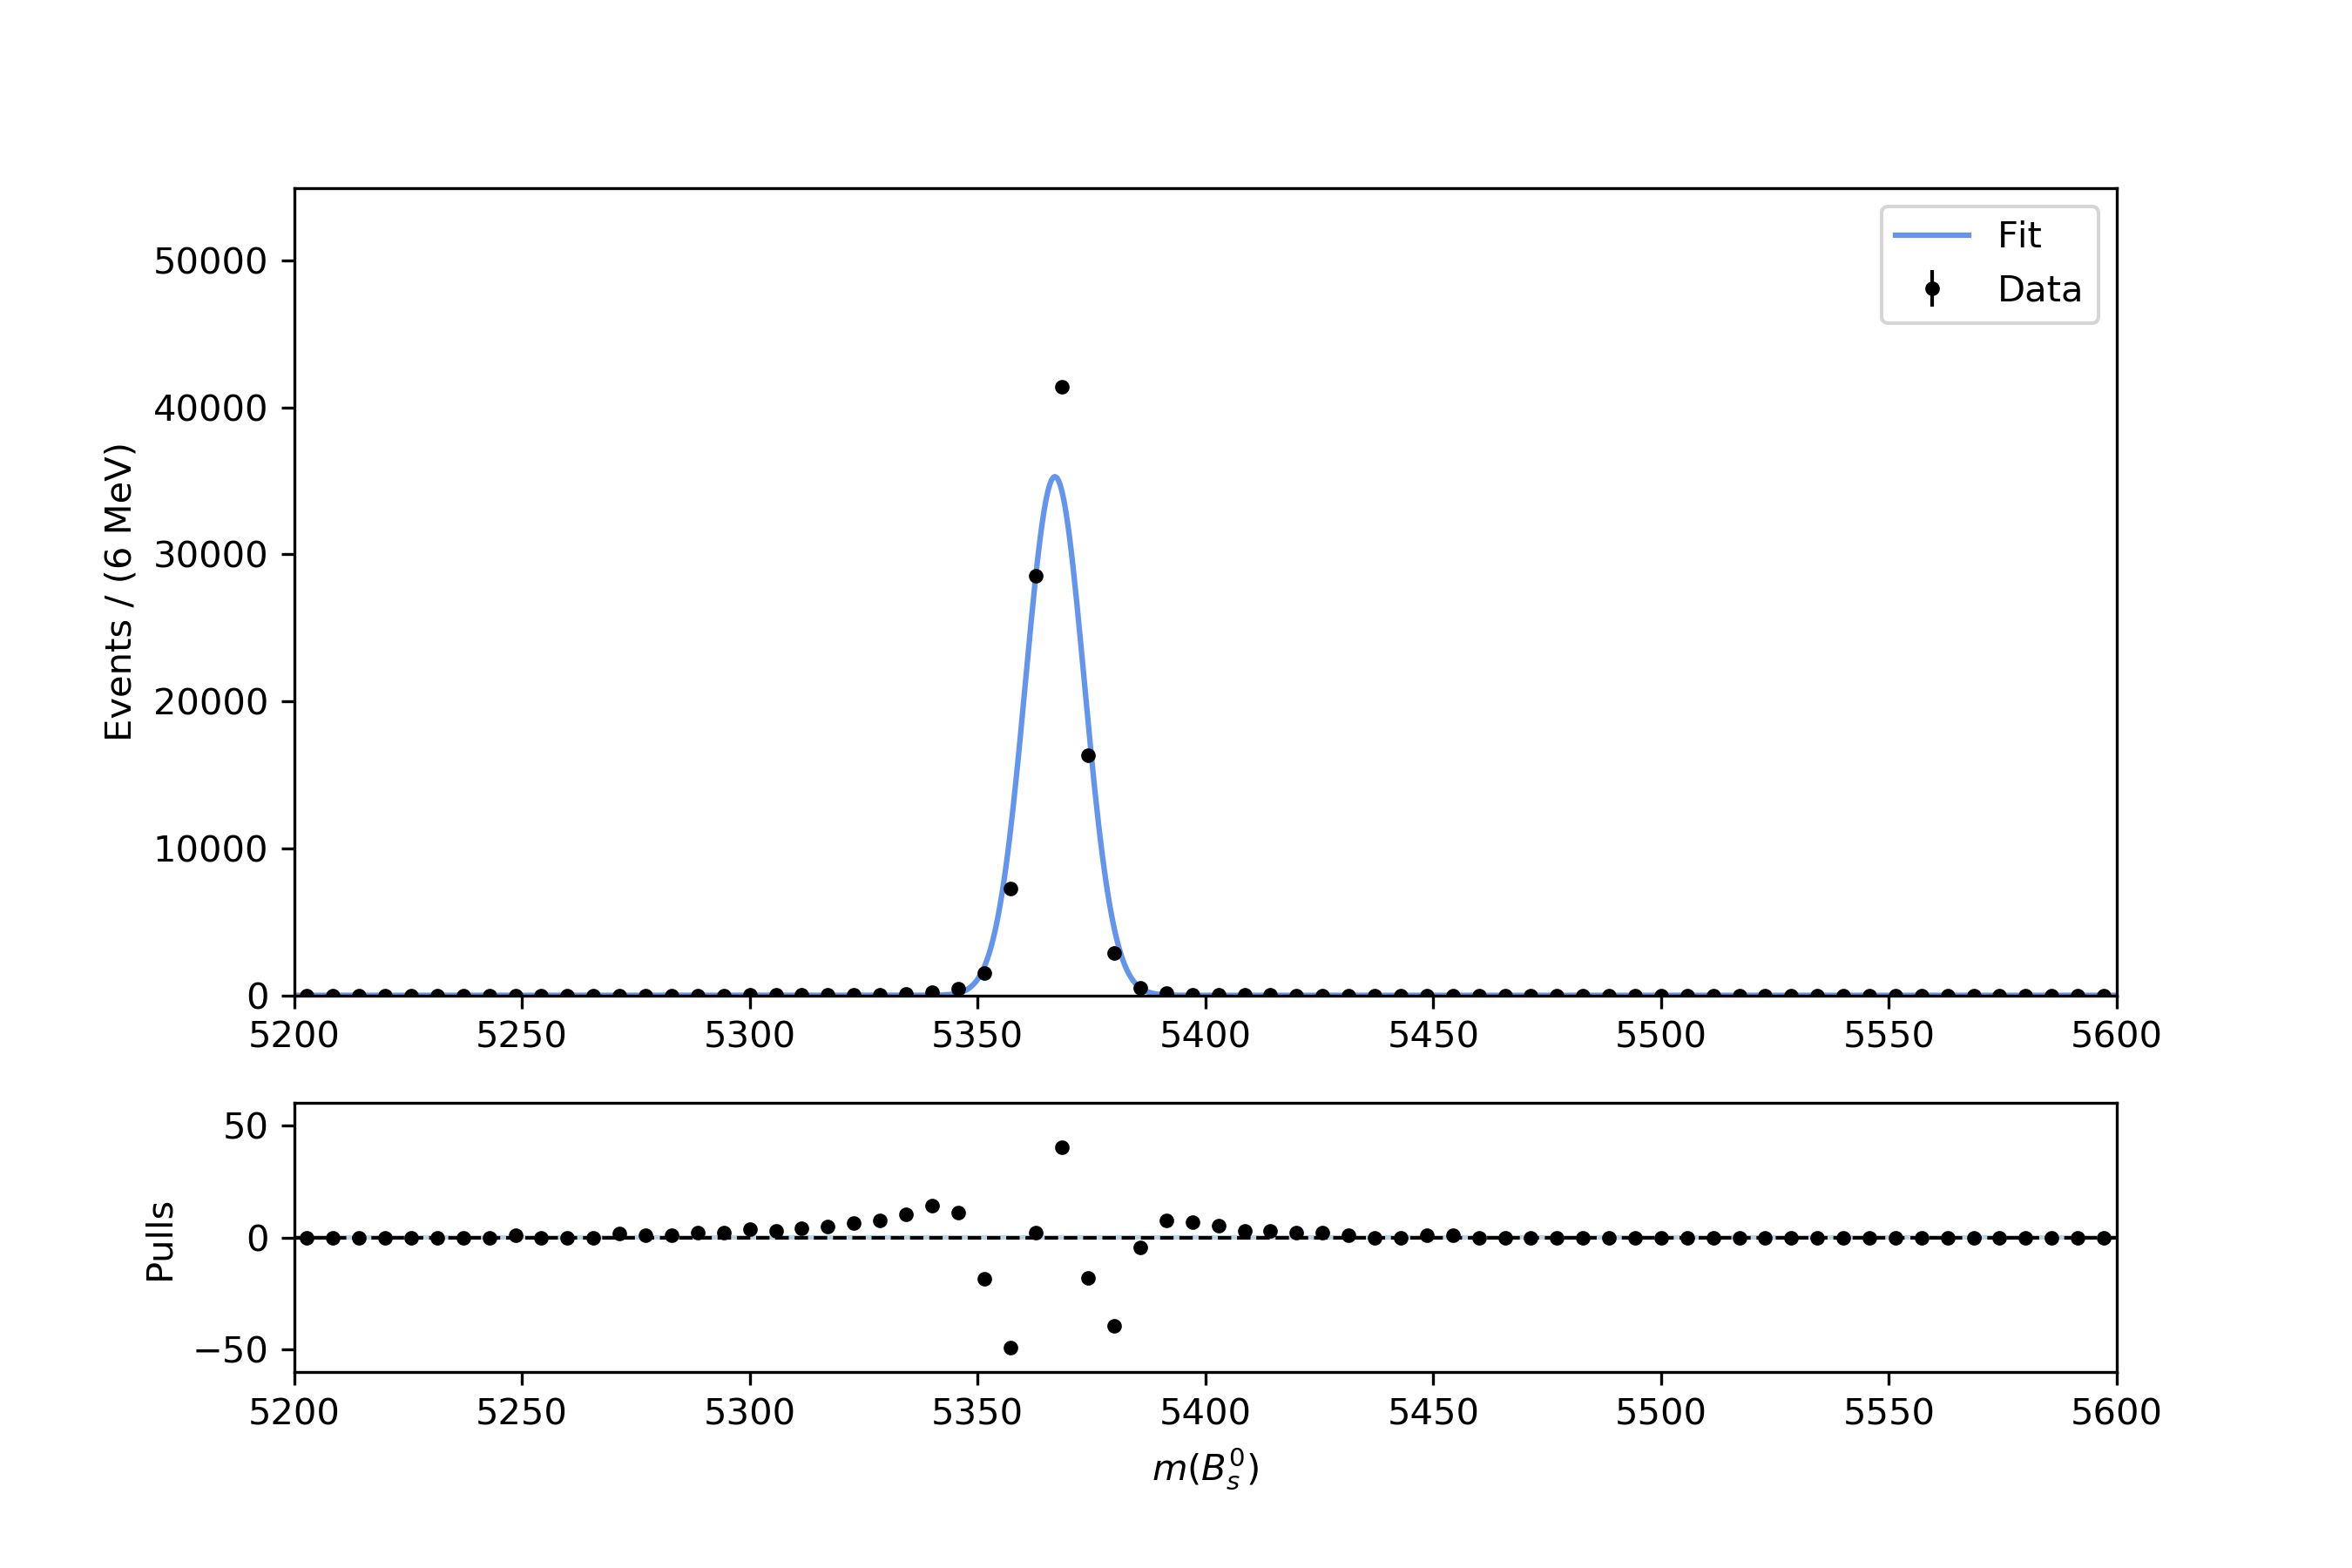
\includegraphics[width=0.99\linewidth]{Figure/second.png}
            \caption{Signal simulation.}
            \label{fit_signal_peak}
        \end{subfigure}
        \hfill
        \begin{subfigure}[b]{0.49\linewidth}
            \centering
            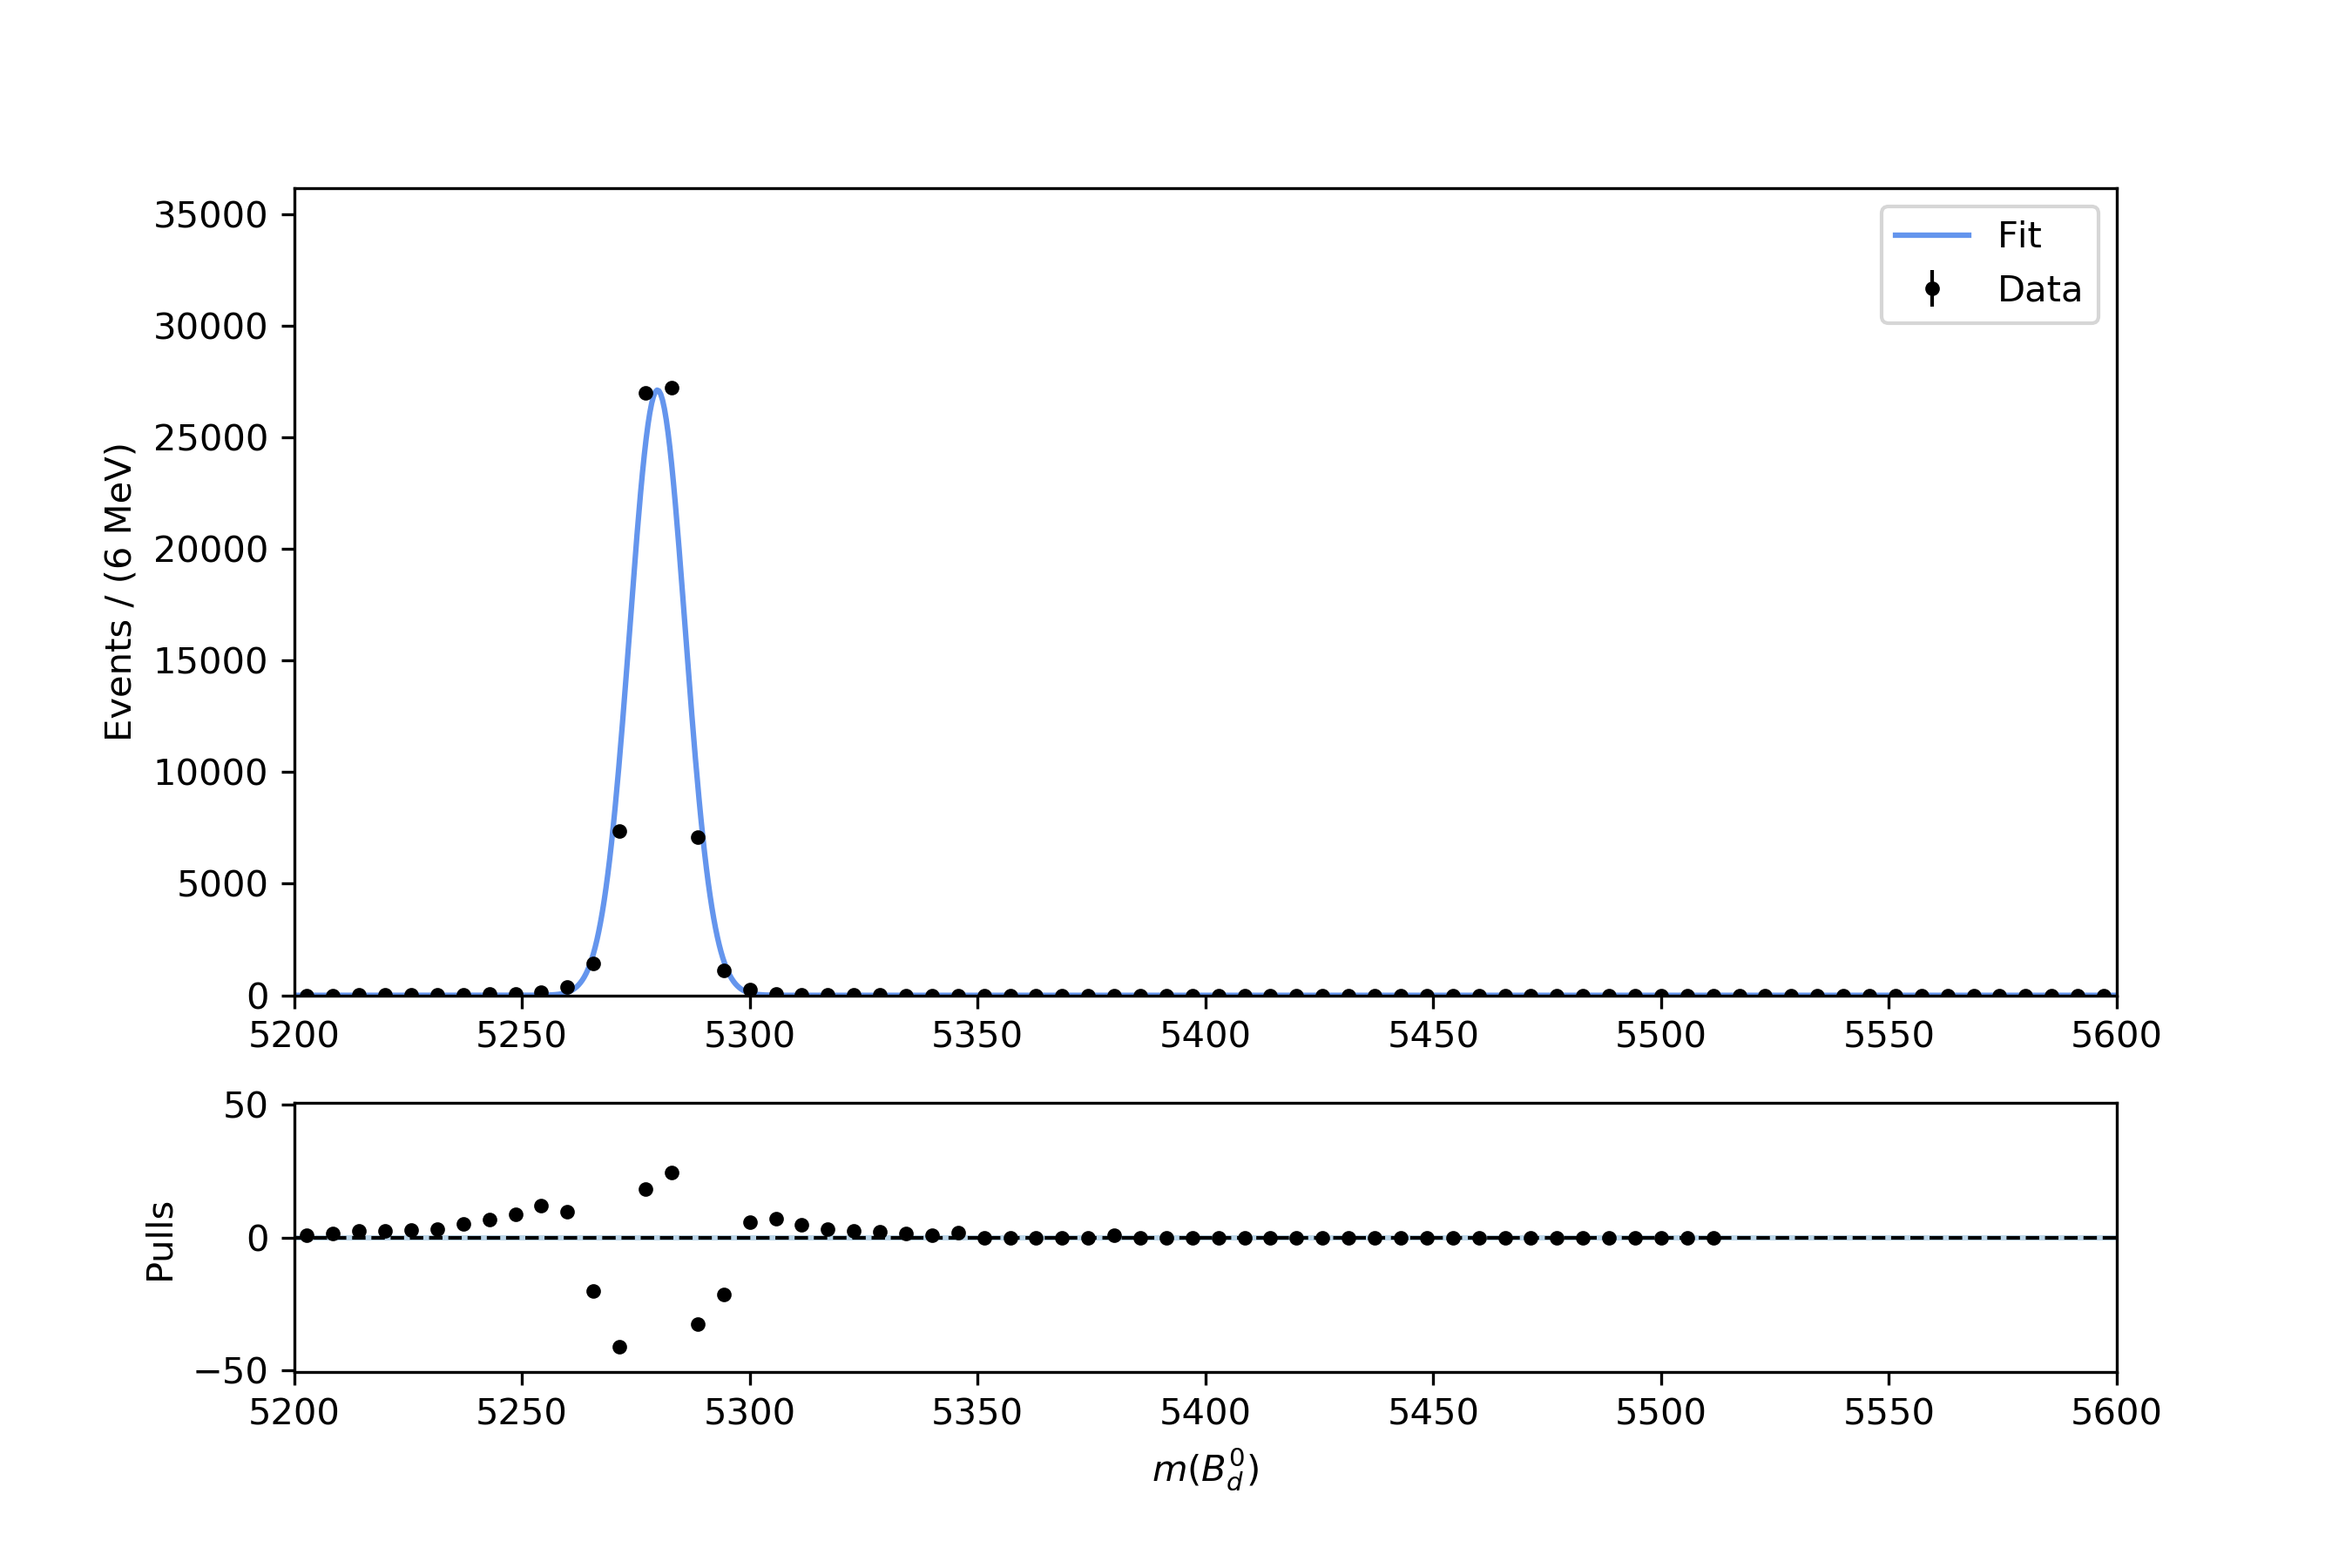
\includegraphics[width=0.99\linewidth]{Figure/third.png}
            \caption{Control simulation.}
            \label{fit_control_peak}
        \end{subfigure}
        \caption{Fitted peak to the signal and control simulation.}
    \end{figure}

    When considering the full mass window of the real data sample, the shapes obtained from the preliminary fits on simulations along with an exponential background are shown in Figure \ref{sec_last}. An exponential background refers to a type of background distribution in data that decays exponentially. This can be represented mathematically as:\\

    \begin{align}
        f(x)=Ae^{-\lambda x}
    \end{align}

    where A is the normalization constant, $\lambda$ is the decay constant and x is the observable.\\
    
    \begin{figure}[H]
        \centering
        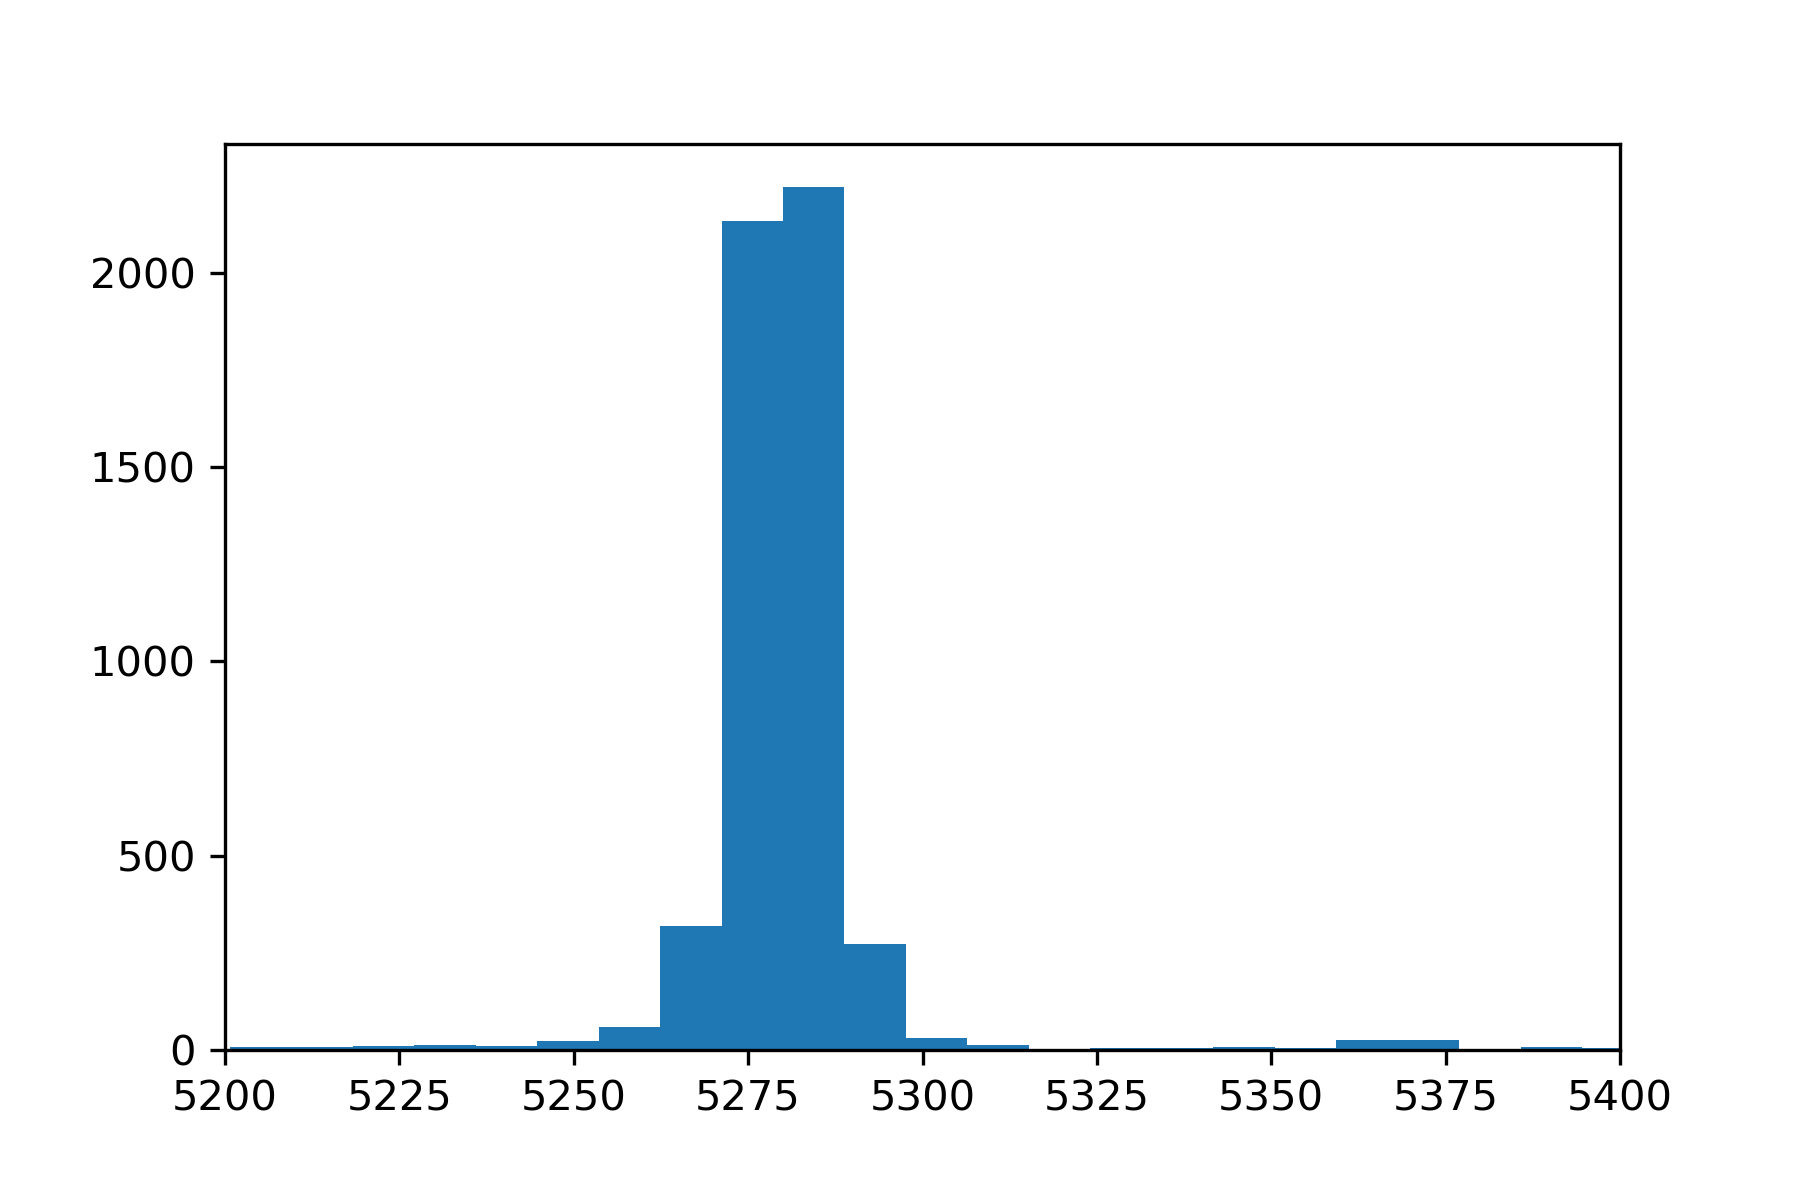
\includegraphics[width=0.8\linewidth]{Figure/second_last.png}
        \caption{Full data fitted with fixed peak shapes and exponential background.}
        \label{sec_last}
    \end{figure}
    Figure \ref{final} shows the invariant mass distribution of candidates from the real data sample which were selected via the classifier criteria. The results of the fit are overlaid.\\
    \begin{figure}[H]
        \centering
        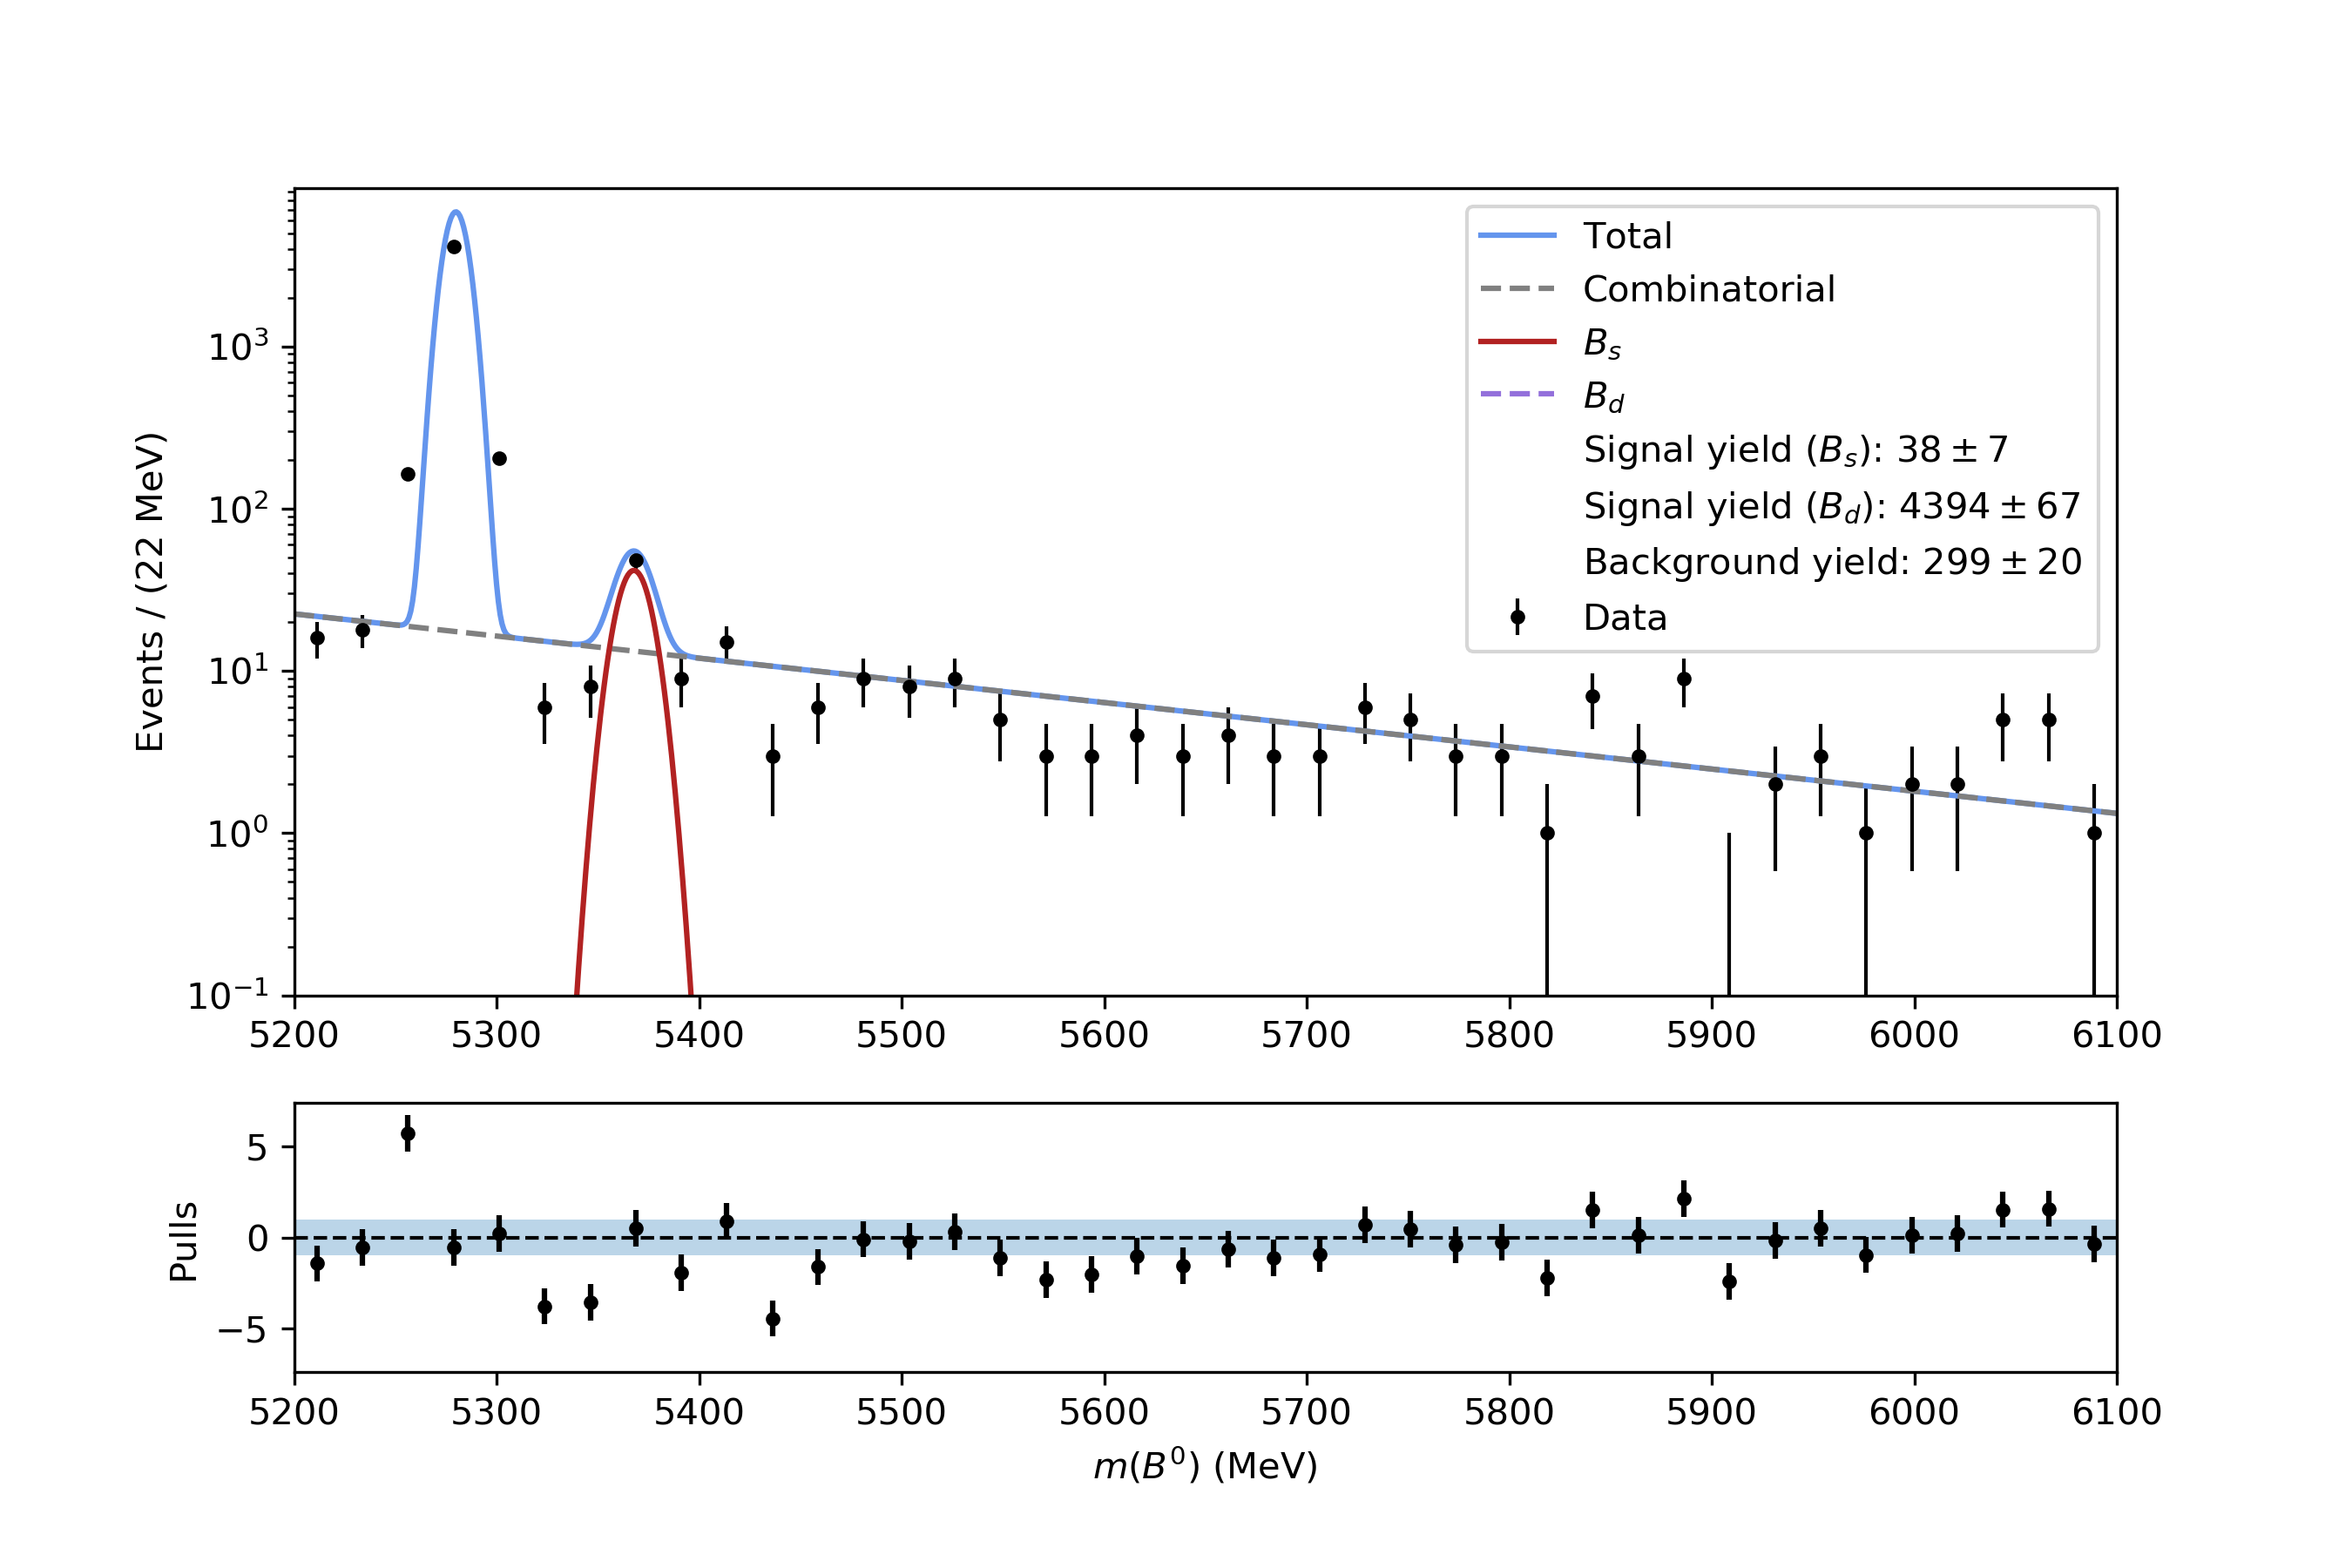
\includegraphics[width=0.8\linewidth]{Figure/final_fit.png}
        \caption{Full mass window of the real dataset using the shapes obtained from the preliminary fits on the simulations and an exponential background.}
        \label{final}
    \end{figure}
    Using the values, obtained from the fit, the proxy significance can be calculated. The signal and background events in the signal region are $n_{sig}=30$ and $n_{bkg}=17$ respectively. Hence, according to Eqn.\ref{proxy}, the signal significance is 4.42.\\
    
% \chapter{Source Code Example}\label{ch4:code}

%%% LaTeX2e file `chap2'
%% generated by the `filecontents' environment
%% from source `main' on 2018/03/29.
%%
\chapter{Discussions}



	


%% LaTeX2e file `chap2'
%% generated by the `filecontents' environment
%% from source `main' on 2018/03/29.
%%
\chapter{Conclusion}\label{ch:conclusion}
The investigation of scintillating fibers for the LHCb SciFi Tracker revealed key insights into their light transmission behavior and structural efficiency. Through both experimental and simulation analyses, the spatial resolution and angular photon distribution were characterized. Simulation data showed strong alignment with theoretical expectations, including attenuation behavior and total internal reflection characteristics for both core and cladding photons. Moreover, the experimental intensity measurements showed consistency with the simulation data. In summary, the simulation results provided a robust understanding, confirming that the optical behavior of the fibers satisfies the design expectations under ideal conditions.\\

% Task1 %


%Task 2%


%Task 3%

%Task 4%

 % Additionally, human error in data handling or interpretation could also contribute.



Therefore, our study strongly supports particle detection using scintillating fibers in high-precision detector systems such as LHCb.




\appendix
% \chapter{Tables}

\begin{table}
\caption{Armadillos}
\label{arm:table}
\begin{center}
\begin{tabular}{||l|l||}\hline
Armadillos & are \\\hline
our	   & friends \\\hline
\end{tabular}
\end{center}
\end{table}

\clearpage
\newpage

% \chapter{Figures}

\vspace*{-3in}

\begin{figure}
%\vspace{2.4in}
\includegraphics[width=0.9\textwidth]{figure/blochvec.png}
\caption{Bloch sphere}
\label{fig1}
\end{figure}
\clearpage
\newpage



%%% This defines the bibliography file (main.bib) and the bibliography style.
%% If you want to create a bibliography file by hand, change the contents of
%% this file to a `thebibliography' environment.  For more information 
%% see section 4.3 of the LaTeX manual.
\begin{singlespace}
\bibliography{main}
\bibliographystyle{plain}
\begin{thebibliography}{99}

\bibitem{nielson} M. A. Nielsen and I. L. Chuang, ``Quantum Computation
and Quantum Information,'' (Cambridge University Press,
Cambridge, England, 2000).

\bibitem{wisemil} H. M. Wiseman and G. J. Milburn, ``Quantum Measurement and Control,'' (Cambridge University Press, Cambridge, UK, 2010).

\bibitem{weber} S. J. Weber, A. Chantasri, J. Dressel, A. N. Jordan, K. W. Murch, and I. Siddiqi, ``Mapping the optimal route between two quantum states,'' Nature (London) {\bf 511}, 570 (2014).

% \bibitem{luis} L. Cortez, A. Chantasri, L. P. Garcia-Pintos, J. Dressel, and A. N. Jordan, ``Rapid estimation of drifting parameters in continuously measured quantum systems,''
% Physical Review A {\bf 95}, 012314 (2017).

\bibitem{lightmode} 
D. T. Smithey \textit{et al}., Phys. Rev. Lett. 70, 1244 (1993); G. Breitenbach \textit{et al}., Nature (London) 387, 471 (1997).



\end{thebibliography}
\end{singlespace}

%\bibliographystyle{abbrv}
\bibliographystyle{plain}
\bibliography{references.bib}
\end{document}

